%%%%%%%%%%%%%%%%%%%%%%%%%%%%%%%%%%%%%%%%%%%%%%%%%%%%%%%%%%%%%%%%%%%%%%%
%%%%%%%%%%%%%%%%%%%%%%%%%%%%%%%%%%%%%%%%%%%%%%%%%%%%%%%%%%%%%%%%%%%%%%%
%%%%%                                                                 %
%%%%%     report.tex                                                  %
%%%%%                                                                 %
%%%%% Author:      Renzo Andri/Matthias Baer                          %
%%%%% Created:     19.11.2013                                         %
%%%%% Description: Implementation and Optimization of the OpenRISC    %
%%%%%              core - Main report file                            %
%%%%%                                                                 %
%%%%%%%%%%%%%%%%%%%%%%%%%%%%%%%%%%%%%%%%%%%%%%%%%%%%%%%%%%%%%%%%%%%%%%%
%%%%%%%%%%%%%%%%%%%%%%%%%%%%%%%%%%%%%%%%%%%%%%%%%%%%%%%%%%%%%%%%%%%%%%%

%%%%%%%%%%%%%%%%%%%%%%%%%%%%%%%%%%%%%%%%%%%%%%%%%%%%%%%%%%%%%%%%%%%%%%%
%%%%%                                                                 %
%%%%%     Document Class                                              %
%%%%%                                                                 %
%%%%%%%%%%%%%%%%%%%%%%%%%%%%%%%%%%%%%%%%%%%%%%%%%%%%%%%%%%%%%%%%%%%%%%%
\documentclass[%
 oneside,      % einseitig => PDF Abgabe. 
% twoside,     % Zweiseitig => Print (reminder: erste seite separat
	       	 % im one-side stil drucken!
 openany,      % Open chapters on odd and even pages.
 halfparskip,  % Create small spaces for new paragraphs but no indents.
]{scrbook}

\usepackage{pdfpages}
%%%%%%%%%%%%%%%%%%%%%%%%%%%%%%%%%%%%%%%%%%%%%%%%%%%%%%%%%%%%%%%%%%%%%%%
%%%%%                                                                 %
%%%%%     Preamble                                                    %
%%%%%                                                                 %
%%%%%%%%%%%%%%%%%%%%%%%%%%%%%%%%%%%%%%%%%%%%%%%%%%%%%%%%%%%%%%%%%%%%%%%
% Load the preamble from another file.
%%%%%%%%%%%%%%%%%%%%%%%%%%%%%%%%%%%%%%%%%%%%%%%%%%%%%%%%%%%%%%%%%%%%%%%
%%%%%%%%%%%%%%%%%%%%%%%%%%%%%%%%%%%%%%%%%%%%%%%%%%%%%%%%%%%%%%%%%%%%%%%
%%%%%                                                                 %
%%%%%     preamble.tex                                                %
%%%%%                                                                 %
%%%%% Author:      Michael Muehlberghuber                             %
%%%%% Created:     01.07.2012                                         %
%%%%% Description: This file contains the preamble of the             %
%%%%%              Semester-/Master-Project LaTeX report example.     %
%%%%%                                                                 %
%%%%% History:                                                        %
%%%%%%%%%%%%%%                                                        %
%%%%% 2012/07/01:  *) Created initial version.                        %
%%%%%                                                                 %
%%%%%%%%%%%%%%%%%%%%%%%%%%%%%%%%%%%%%%%%%%%%%%%%%%%%%%%%%%%%%%%%%%%%%%%
%%%%%%%%%%%%%%%%%%%%%%%%%%%%%%%%%%%%%%%%%%%%%%%%%%%%%%%%%%%%%%%%%%%%%%%

%%%%%%%%%%%%%%%%%%%%%%%%%%%%%%%%%%%%%%%%%%%%%%%%%%%%%%%%%%%%%%%%%%%%%%%
%%%%%                                                                 %
%%%%%     Package Loading                                             %
%%%%%                                                                 %
%%%%%%%%%%%%%%%%%%%%%%%%%%%%%%%%%%%%%%%%%%%%%%%%%%%%%%%%%%%%%%%%%%%%%%%

% Determines the input encoding.
\usepackage[%
 utf8,
% latin1
]{inputenc}

% ---------------------------------------------------------------------

% Determines the output encoding.
\usepackage[T1]{fontenc}

% ---------------------------------------------------------------------

% Determines language settings.
\usepackage[%
 english    % You may change this to 'ngerman' in order to write a
            % german report.
]{babel}

% ---------------------------------------------------------------------

% Provides image loading.
\usepackage{graphicx}

% ---------------------------------------------------------------------

% Provides customization of chapter headings.
\usepackage[%
	Lenny     % Choose a nice layout for chapter headings.
]{fncychap}

% ---------------------------------------------------------------------

% Provides some blindtext.
\usepackage{lipsum}

% ---------------------------------------------------------------------

% Provides stretchable tables.
\usepackage{tabularx}

% ---------------------------------------------------------------------

% Provides some fancy boxes.
\usepackage{fancybox}

% ---------------------------------------------------------------------

% Provides subfigures.
\usepackage{subcaption}

% ---------------------------------------------------------------------

% Provides colors in LaTeX.
\usepackage{xcolor}

% ---------------------------------------------------------------------

% Provides conditionals (for titlepage).
\usepackage{xifthen}

% ---------------------------------------------------------------------

% Provides the algorithm environment
\usepackage[ruled,%
            linesnumbered]{algorithm2e}

% ---------------------------------------------------------------------

% Provides bold greek math symbols.
\usepackage{bm}

% ---------------------------------------------------------------------

% Allows to include pdf documents.
\usepackage{pdfpages}

% ---------------------------------------------------------------------

% Provides nicer tables than the standard tables.
\usepackage{booktabs}

% ---------------------------------------------------------------------

% Provides simple line spacings.
\usepackage{setspace}

% ---------------------------------------------------------------------

% Provides simple line spacings.
\usepackage{geometry}

% ---------------------------------------------------------------------

% Provides more customizeable captions.
\usepackage{capt-of}

% ---------------------------------------------------------------------

% Provides small table of contents (e.g., for single chapters or the
% appendix).
\usepackage{minitoc}

% ---------------------------------------------------------------------

% Provides a simple command to describe a directory tree.
\usepackage{dirtree}

% ---------------------------------------------------------------------

%%%%%                                                             %%%%%
%%%%% ATTENTION: Loading further packagaes should go in here.     %%%%%
%%%%%                                                             %%%%%

% ---------------------------------------------------------------------

% Provides hyperlinks within your document. Should always be loaded at
% the end.
\usepackage{hyperref}

% ---------------------------------------------------------------------

% Provides multiple glossaries (incl. list acronyms, list of symbols,
% etc.).
\usepackage[%
 toc,              % Add the glossaries to the table of contents.
 acronym,          % Add a list of acronyms.
 section=chapter,  % Show glossary headers as chapters.
 nonumberlist,     % Do not print the page numbers next to glossary
                   % entries.
]{glossaries}


\usepackage{float}
\usepackage{amsmath}
\usepackage{threeparttable}
\usepackage{fancyvrb}
\usepackage{listings}
\usepackage{pdflscape}
% Tikz/plots
\usepackage{tikz}
\usetikzlibrary{backgrounds}
\usepackage{pgfplots}
\usetikzlibrary{pgfplots.groupplots}

\pgfplotscreateplotcyclelist{mylist}{ 
  fill=gray!20,draw=black!90,line width=.2pt\\%
  fill=blue!60,draw=black!90,line width=.2pt\\%
  fill=red!60,draw=black!90,line width=.2pt\\%
  fill=orange!60,draw=black!90,line width=.2pt\\%
  fill=yellow!60,draw=black!90,line width=.2pt\\%
  fill=green!60,draw=black!90,line width=.2pt\\%
  fill=brown!60,draw=black!90,line width=.2pt\\%
  fill=black!60,draw=black!90,line width=.2pt\\%
  fill=white\\%
}
\newcommand\drawbar[1]{%
  \begin{tikzpicture}%
    \draw[fill=#1,draw=black!90,ultra thin] (0pt,0pt) rectangle (3pt,8pt);%
    \draw[fill=#1,draw=black!90,ultra thin] (6pt,0pt) rectangle (9pt,6pt);%
  \end{tikzpicture}\hspace{0pt}%
}


%%%%%%%%%%%%%%%%%%%%%%%%%%%%%%%%%%%%%%%%%%%%%%%%%%%%%%%%%%%%%%%%%%%%%%%
%%%%%                                                                 %
%%%%%     Custom Settings                                             %
%%%%%                                                                 %
%%%%%%%%%%%%%%%%%%%%%%%%%%%%%%%%%%%%%%%%%%%%%%%%%%%%%%%%%%%%%%%%%%%%%%%
% Do not use sans-serif fonts for all dispositions (chapters,
% sections, etc.)
\setkomafont{disposition}{\normalfont\bfseries}


%%%%%%%%%%%%%%%%%%%%%%%%%%%%%%%%%%%%%%%%%%%%%%%%%%%%%%%%%%%%%%%%%%%%%%%
%%%%%                                                                 %
%%%%%     Custom Macros                                               %
%%%%%                                                                 %
%%%%%%%%%%%%%%%%%%%%%%%%%%%%%%%%%%%%%%%%%%%%%%%%%%%%%%%%%%%%%%%%%%%%%%%
% Create an inline command for shell commands.
\newcommand{\shell}[1]{\texttt{#1}}

% Create an enviroment for a shell commands.
\newenvironment{shellenv}%
{\VerbatimEnvironment%
 \begin{Sbox}\begin{minipage}{0.97\textwidth}\begin{Verbatim}%
}%
{\end{Verbatim}\end{minipage}\end{Sbox}%
\setlength{\fboxsep}{6pt}\shadowbox{\TheSbox}}%

% Create an inline command for files.
\newcommand{\file}[1]{\texttt{#1}}

% Create a command for command parameters.
\newcommand{\parameter}[1]{$<$#1$>$}

\newcommand{\instr}[1]{\texttt{#1}}


\definecolor{lightGray}{RGB}{240,240,240}

\lstnewenvironment{instrenv}{\lstset{backgroundcolor=\color{lightGray},frame=single,basicstyle=\ttfamily}}{}

\newcommand{\orion}{\textsc{Or10n}\xspace}


%%%%%%%%%%%%%%%%%%%%%%%%%%%%%%%%%%%%%%%%%%%%%%%%%%%%%%%%%%%%%%%%%%%%%%%
%%%%%                                                                 %
%%%%%     Titlepage Macros - !!! DO NOT CHANGE !!!                    %
%%%%%                                                                 %
%%%%%%%%%%%%%%%%%%%%%%%%%%%%%%%%%%%%%%%%%%%%%%%%%%%%%%%%%%%%%%%%%%%%%%%
% Create a command for missing title page parameters.
\newcommand{\misspar}[1]{\textcolor{red}{\textbf{$<$#1$>$}}}

\makeatletter

% Redefine existing class macros as missing.
\title{\misspar{Specify Title}}%
\author{\misspar{Specify Author}}%
\date{\misspar{Specify Date}}%

% Define a command for setting the semester on the titlepage.
\def\@semester{\misspar{Specify Semester}}%
\newcommand{\setsemester}[1]{\def\@semester{#1}}%
\let\semester\setsemester%
\newcommand{\show@semester}{\@semester}%

% Define a command for setting the type of the report (Master Thesis,
% Semester Project, etc.) on the titlepage.
\def\@reporttype{\misspar{Specify Report Type}}%
\newcommand{\setreporttype}[1]{\def\@reporttype{#1}}%
\let\reporttype\setreporttype%
\newcommand{\show@reporttype}{\@reporttype}%

% Define a command for setting the image path for the image on the
% titlepage.
\def\@titlelogo{}%
\newcommand{\settitlelogo}[1]{\def\@titlelogo{#1}}%
\let\titlelogo\settitlelogo%

% Define a command for setting the image height on the titlepage.
\def\@logoheight{7cm}%
\newcommand{\setlogoheight}[1]{\def\@logoheight{#1}}%
\let\logoheight\setlogoheight%
\newcommand{\show@logoheight}{\@logoheight}%

% Define a command for setting the email on the titlepage.
\def\@email{\misspar{Specify E-Mail}}%
\newcommand{\setemail}[1]{\def\@email{#1}}%
\let\email\setemail%
\newcommand{\show@email}{\@email}%

% Define a command for setting the first supervisor on the titlepage.
\def\@firstsup{\misspar{Specify First Supervisor}}%
\newcommand{\setfirstsup}[1]{\def\@firstsup{#1}}%
\let\firstsup\setfirstsup%
\newcommand{\show@firstsup}{\@firstsup}%

% Define a command for setting the second supervisor on the titlepage.
\def\@secondsup{\misspar{Specify Second Supervisor}}%
\newcommand{\setsecondsup}[1]{\def\@secondsup{#1}}%
\let\secondsup\setsecondsup%
\newcommand{\show@secondsup}{\@secondsup}%

% Define a command for setting the professor on the titlepage.
\def\@professor{\misspar{Specify Professor}}%
\newcommand{\setprofessor}[1]{\def\@professor{#1}}%
\let\professor\setprofessor%
\newcommand{\show@professor}{\@professor}%

% Define a command for setting the margin on the title page.
\def\@titlepagemargin{3cm}%
\newcommand{\settitlepagemargin}[1]{\def\@titlepagemargin{#1}}%
\let\titlepagemargin\settitlepagemargin%
\newcommand{\show@titlepagemargin}{\@titlepagemargin}%

\makeatother


%%%%%
%%%%% Load the glossaries.
%%%%%
%%%%%%%%%%%%%%%%%%%%%%%%%%%%%%%%%%%%%%%%%%%%%%%%%%%%%%%%%%%%%%%%%%%%%%%
%%%%%                                                                 %
%%%%%     Make Glossaries                                             %
%%%%%                                                                 %
%%%%%%%%%%%%%%%%%%%%%%%%%%%%%%%%%%%%%%%%%%%%%%%%%%%%%%%%%%%%%%%%%%%%%%%

% Required to generate the index for the glossaries.
\makeglossaries

%%%%%%%%%%%%%%%%%%%%%%%%%%%%%%%%%%%%%%%%%%%%%%%%%%%%%%%%%%%%%%%%%%%%%%
%%%%%                                                                %
%%%%%     Definitions of all glossary entries which will appear in   %
%%%%%     the default (main) glossary.                               %
%%%%%                                                                %
%%%%%%%%%%%%%%%%%%%%%%%%%%%%%%%%%%%%%%%%%%%%%%%%%%%%%%%%%%%%%%%%%%%%%%

\newglossaryentry{monkey}{name=Monkey,description={Lorem ipsum dolor
sit amet, consetetur sadipscing elitr, sed diam nonumy eirmod tempor
invidunt ut labore et dolore magna aliquyam erat, sed diam
voluptua. At vero eos et accusam et justo duo dolores et ea
rebum. Stet clita kasd gubergren, no sea takimata sanctus est Lorem
ipsum dolor sit amet}}


% Add all glossary entries to the glossary, even if they have not been
% referenced.
%\glsaddall[types={main}]


%%%%%%%%%%%%%%%%%%%%%%%%%%%%%%%%%%%%%%%%%%%%%%%%%%%%%%%%%%%%%%%%%%%%%%
%%%%%                                                                %
%%%%%     Definitions of all acronyms which will appear in the list  %
%%%%%     of acronyms.                                               %
%%%%%                                                                %
%%%%%%%%%%%%%%%%%%%%%%%%%%%%%%%%%%%%%%%%%%%%%%%%%%%%%%%%%%%%%%%%%%%%%%

\newacronym{iis}{IIS}{Integrated Systems Laboratory}
\newacronym{ASIC}{ASIC}{Application-Specific Integrated Circuit}
\newacronym{fpga}{FPGA}{Field Programmable Gate Array}
\newacronym{LED}{LED}{Light-Emitting Diode}
\newacronym{JTAG}{JTAG}{Joint Test Action Group}
\newacronym{nist}{NIST}{National Institute of Standards and
Technology}
\newacronym{aes}{AES}{Advanced Encryption Standard}
\newacronym{ecc}{ECC}{Elliptic Curve Cryptography}
\newacronym{ecdsa}{ECDSA}{Elliptic Curve Digital Signature Algorithm}
\newacronym{des}{DES}{Data Encryption Standard}
\newacronym{wysiwyg}{WYSIWYG}{What You See Is What You Get}
\newacronym{pdf}{PDF}{Portable Document Format}
\newacronym{eps}{EPS}{Encapsulated PostScript}
\newacronym{dvi}{DVI}{Device Independent File Format }
\newacronym{ic}{IC}{Integrated Circuit}

\newacronym{PULP}{PULP}{Parallel Ultra-Low-Power Processing-Platform}
\newacronym{TCDM}{TCDM}{Tightly-Coupled Data Memory}
\newacronym{ROM}{ROM}{Read-Only Memory}
\newacronym{RAM}{RAM}{Random-Access Memory}
\newacronym{SPI}{SPI}{Serial Peripheral Interface}
\newacronym{UART}{UART}{Universal Asynchronous Receiver Transmitter}
\newacronym{SRAM}{SRAM}{Static Random-Access Memory}
\newacronym{SCM}{SCM}{Standard-Cell Memory}
\newacronym{LSU}{LSU}{Load-and-Store Unit}

\newacronym{IPC}{IPC}{Instructions per Cycle}
\newacronym{CPU}{CPU}{Central Processing Unit}
\newacronym{SoC}{SoC}{System-on-a-Chip}
\newacronym{DMA}{DMA}{Direct Memory Access}

\newacronym{FSM}{FSM}{Finite State Machine}

\newacronym{IF}{IF}{Instruction Fetch}
\newacronym{ID}{ID}{Instruction Decode}
\newacronym{EX}{EX}{Execute}
\newacronym{WB}{WB}{Write Back}
\newacronym{SPR}{SPR}{Special-Purpose Register}
\newacronym{GPR}{GPR}{General-Purpose Register}
\newacronym{ISA}{ISA}{Instruction Set Architecture}
\newacronym{RISC}{RISC}{Reduced Instruction Set Computer}
\newacronym{ALU}{ALU}{Arithmetic Logic Unit}
\newacronym{MAC}{MAC}{Multiply-Accumulate}
\newacronym{SIMD}{SIMD}{Single Instruction Multiple Data}

\newacronym{GCC}{GCC}{GNU Compiler Collection}

\newacronym{LSB}{LSB}{Least Significant Bit}
\newacronym{MSB}{MSB}{Most Significant Bit}

\newacronym{FIR}{FIR}{Finite Impulse Response}

% Add all acronyms to the list of acronyms even if they have not been
% referenced.
%\glsaddall[types={\acronymtype}]


% Define which source files should actually been processed.
%\includeonly{./content/06-design_implementation}


%%%%%%%%%%%%%%%%%%%%%%%%%%%%%%%%%%%%%%%%%%%%%%%%%%%%%%%%%%%%%%%%%%%%%%%
%%%%%                                                                 %
%%%%%     Document Settings                                           %
%%%%%                                                                 %
%%%%%%%%%%%%%%%%%%%%%%%%%%%%%%%%%%%%%%%%%%%%%%%%%%%%%%%%%%%%%%%%%%%%%%%

%%%%% Mandatory title page settings.
\title{Implemenation and Optimization of the OpenRISC Processor}
\author{Renzo Andri\\Matthias Baer}
\email{andrire@student.ethz.ch\\baermatt@student.ethz.ch}
\date{December 2013}
\semester{Autumn Term 2013}
\reporttype{Semester Project}
\firstsup{Dr. Frank Kagan G\"urkaynak, kgf@ee.ethz.ch}
\secondsup{Michael Gautschi, gautschi@iis.ee.ethz.ch}
\professor{Prof. Dr. Luca Benini, lbenini@iis.ee.ethz.ch}

%%%%% Optional title page settings.
\titlelogo{./figures/or10n_layout_small}  % Title page logo path.
\logoheight{7cm}                      % Height of the title page logo.
\titlepagemargin{3cm}                 % Margin on the title page.


%%%%%%%%%%%%%%%%%%%%%%%%%%%%%%%%%%%%%%%%%%%%%%%%%%%%%%%%%%%%%%%%%%%%%%%
%%%%%                                                                 %
%%%%%     Start of Document                                           %
%%%%%                                                                 %
%%%%%%%%%%%%%%%%%%%%%%%%%%%%%%%%%%%%%%%%%%%%%%%%%%%%%%%%%%%%%%%%%%%%%%%
\begin{document}

% Prepare document for minitoc insertions.
\dominitoc
\dominilof

\frontmatter

% Create title.
\input{./content/00_0_title}
%\maketitle

% Include acknowledgements, abstract, etc...
%%%%%%%%%%%%%%%%%%%%%%%%%%%%%%%%%%%%%%%%%%%%%%%%%%%%%%%%%%%%%%%%%%%%%%%
%%%%%%%%%%%%%%%%%%%%%%%%%%%%%%%%%%%%%%%%%%%%%%%%%%%%%%%%%%%%%%%%%%%%%%%
%%%%%                                                                 %
%%%%%     <file_name>.tex                                             %
%%%%%                                                                 %
%%%%% Author:      <author>                                           %
%%%%% Created:     <date>                                             %
%%%%% Description: <description>                                      %
%%%%%                                                                 %
%%%%%%%%%%%%%%%%%%%%%%%%%%%%%%%%%%%%%%%%%%%%%%%%%%%%%%%%%%%%%%%%%%%%%%%
%%%%%%%%%%%%%%%%%%%%%%%%%%%%%%%%%%%%%%%%%%%%%%%%%%%%%%%%%%%%%%%%%%%%%%%

\chapter*{Acknowledgements}
%TODO

I would like to thank my supervisors Michael Gautschi, Antonio Pullini and Luca
Benini for giving me the opportunity to work on such a huge project and for
their advice during the course of this thesis.
I want to thank Eric Flamand for his work on proposing instruction set
extensions for OpenRISC and his support during evaluation and implementation in
RTL.
For his work on the LLVM compiler support for our platform and advice during
the evaluation of possible extensions I would like to thank Michele Beretta,
who was also a source of inspiration for ideas on how to improve our platform
in terms of infrastructure.
For his helpful advice and infrastructure support at ETH I would like to thank
Frank G\"urkaynak,
and last but not least everyone else in the PULP team and in the Integrated
Systems Lab that has supported me during this thesis.

%%%%%%%%%%%%%%%%%%%%%%%%%%%%%%%%%%%%%%%%%%%%%%%%%%%%%%%%%%%%%%%%%%%%%%%
%%%%%%%%%%%%%%%%%%%%%%%%%%%%%%%%%%%%%%%%%%%%%%%%%%%%%%%%%%%%%%%%%%%%%%%
%%%%%                                                                 %
%%%%%     00_2_abstract.tex                                           %
%%%%%                                                                 %
%%%%% Author:      <author>                                           %
%%%%% Created:     <date>                                             %
%%%%% Description: <description>                                      %
%%%%%                                                                 %
%%%%%%%%%%%%%%%%%%%%%%%%%%%%%%%%%%%%%%%%%%%%%%%%%%%%%%%%%%%%%%%%%%%%%%%
%%%%%%%%%%%%%%%%%%%%%%%%%%%%%%%%%%%%%%%%%%%%%%%%%%%%%%%%%%%%%%%%%%%%%%%

\chapter*{Abstract}
Today's embedded devices like wearables, smartphones, Internet of Things
devices and sensors need a vast amount of computing power in a very constrained
environment where only a limited amount of energy is available.
By reducing the operating voltage of digital circuits to near-threshold values,
the energy efficiency of those circuits can be improved. To recover the loss in
speed, parallelization can be employed.

In our Parallel Ultra-Low power Processor (PULP), several OpenRISC based cores
are organized in clusters to perform computations in parallel. To increase
their energy efficiency at low voltages even further, the instruction set of
those cores was extended by adding vectorial instructions, bit counting
operations and improvements to the MAC unit. In previous work, extensions for
hardware loops and auto-incrementing load and store instructions were added to
the core on which the new instructions are built on. With those extensions, the
cores are able to perform more computations per cycle and thus need to stay
active for a shorter period of time. At the same time the core area has only
increased by $25\%$, while the area of one PULP cluster has increased by $2\%$
due to our additions.
The critical path delay of the core was unaffected by the extensions.

Compared to the original OpenRISC instruction set, a performance gain of up to
a factor of 5x was achieved. In terms of energy efficiency we were able to be
$45\%$ more energy efficient on average.


\include{./content/00_3_authorship}

% Insert table of contents, list of figures, and list of tables.
\tableofcontents
\mtcaddchapter % minitoc fix


\listoffigures
\listoftables
\mtcaddchapter % minitoc fix

% Print list of acronyms.
\setlength{\glslistdottedwidth}{0.2\linewidth}
\printglossary[type=\acronymtype,style=listdotted,title=List of Acronyms]

\include{./content/00_4_conventions}

%%%%%
%%%%% Start the actual main content part.
%%%%%
\mainmatter

% Include the actual content files.
%%%%%%%%%%%%%%%%%%%%%%%%%%%%%%%%%%%%%%%%%%%%%%%%%%%%%%%%%%%%%%%%%%%%%%%
%%%%%%%%%%%%%%%%%%%%%%%%%%%%%%%%%%%%%%%%%%%%%%%%%%%%%%%%%%%%%%%%%%%%%%%
%%%%%                                                                 %
%%%%%     <file_name>.tex                                             %
%%%%%                                                                 %
%%%%% Author:      <author>                                           %
%%%%% Created:     <date>                                             %
%%%%% Description: <description>                                      %
%%%%%                                                                 %
%%%%%%%%%%%%%%%%%%%%%%%%%%%%%%%%%%%%%%%%%%%%%%%%%%%%%%%%%%%%%%%%%%%%%%%
%%%%%%%%%%%%%%%%%%%%%%%%%%%%%%%%%%%%%%%%%%%%%%%%%%%%%%%%%%%%%%%%%%%%%%%

\chapter{Introduction}

Microprocessors for Internet of Things devices, wearables, smartphones, sensors and
medical devices have to work in very energy constrained environments while at
the same time providing a high amount of processing power.
Energy efficiency is thus essential for those kind of devices.
The energy needed for a certain application is the product of the power needed
during its execution and the time required to execute it.

Power consumption can be reduced by operating the digital circuit at the most
energy efficient operating point. This operating point lies near the threshold
voltage of the technology at hand \cite{NTC} as dynamic power scales
quadratically with the supply voltage. Lowering the supply voltage to
near-threshold values leads to an inevitable increase in leakage which
eventually dominates the energy consumption of the circuit, see
Figure~\ref{fig:dyn_leakage} for an example on a 32nm technology \cite{VIVEK}.
One thus has to balance between dynamic energy and leakage. At this operating
point the circuit will only achieve a low frequency compared to higher supply
voltages, which means that the performance will decrease and thus the time that
the circuit needs to be active gets longer. To reduce the active time while not
increasing the power consumption overproportionally, multiple cores can be used
that share the common infrastructure like instruction caches, scratchpad memory
and peripherals. Since the performance of the core has a direct impact on the
time our circuit needs to be active, increasing it can lead to a higher energy
efficiency of the whole system.

\begin{figure}[H]
  \centering \includegraphics[width=0.7\textwidth]{./figures/dyn_leakage}
  \caption{Dynamic vs. leakage energy.}
  \label{fig:dyn_leakage}
\end{figure}

It is the goal of this thesis to increase the energy efficiency and performance
of the \orion core by adding specialized instructions. Those instructions allow
to perform more computations per clock cycle and thus the core needs less time
to process its workload.
Our goal was to add instructions to the OpenRISC \gls{ISA} that add little
overhead in terms of area and pipeline stage delay and thus have little impact
on the energy efficiency and performance when those new instructions are not
used. Since we are working on a many-core cluster platform, it was important
that our changes also work well in this cluster environment. Our focus lay on
adding vectorial support to exploit sub-word parallelism and multiplier
improvements to make the commonly used multiplication operations as fast as
possible. Together with previous \gls{ISA} extensions we achieved a speedup of
up to 5x when using those extensions. Additionally we added bit counting
instructions which can speed up some specific applications up to 35x.

Since this OpenRISC core is used in many projects that are produced as
\glspl{ASIC}, we also wanted to add some features that are usually present in
modern \glspl{CPU}. For example we have added interrupt support and in-circuit
debugging facilities.

This report is structured as follows. In Chapter~\ref{chapter:background} 
background about the platform which was used for this thesis is given.
In Chapter~\ref{chapter:related_work} an overview over related work is
presented.
In Chapter~\ref{chapter:vectorial} the changes to the \gls{ISA} are explained
and  implementation details are given, while the encoding and semantics of
the new instructions are available in Appendix~\ref{chap:instr_encoding}.
In Chapter~\ref{chapter:debug} the debug facilities that were added to the core
are described.
Chapter~\ref{chapter:changes} highlights the microarchitectural changes that
were performed.
In Chapter~\ref{chapter:results} we compare our results of the improved \orion
core with the industry standard ARM Cortex M4 and the old OR1200 OpenRISC core.
Finally Chapter~\ref{chapter:conclusion} draws a conclusion over the changes
that were done to the core during this thesis while
Chapter~\ref{chapter:outlook} gives an outlook over future work.



%%% Local Variables: 
%%% mode: latex
%%% TeX-master: "../report_template"
%%% End: 
 \cleardoublepage
\include{./content/02_preliminaries} \cleardoublepage
%%%%%%%%%%%%%%%%%%%%%%%%%%%%%%%%%%%%%%%%%%%%%%%%%%%%%%%%%%%%%%%%%%%%%%%
%%%%%%%%%%%%%%%%%%%%%%%%%%%%%%%%%%%%%%%%%%%%%%%%%%%%%%%%%%%%%%%%%%%%%%%
%%%%%                                                                 %
%%%%%     <file_name>.tex                                             %
%%%%%                                                                 %
%%%%% Author:      <author>                                           %
%%%%% Created:     <date>                                             %
%%%%% Description: <description>                                      %
%%%%%                                                                 %
%%%%%%%%%%%%%%%%%%%%%%%%%%%%%%%%%%%%%%%%%%%%%%%%%%%%%%%%%%%%%%%%%%%%%%%
%%%%%%%%%%%%%%%%%%%%%%%%%%%%%%%%%%%%%%%%%%%%%%%%%%%%%%%%%%%%%%%%%%%%%%%

\chapter{Related Work}

\label{chapter:related_work}


\section{Hardware Loops \& Auto-Incrementing Load/Stores}
\label{sec:or10n_hwlp_prepost}

The \gls{PULP} team has already extended the OpenRISC \gls{ISA} prior to this
thesis, i.e. zero-overhead hardware loops and extended addressing modes for load
and store operations were added.

Hardware loops eliminate the need of explicitly stating branch instructions
and decreasing the loop counter, instead this is done automatically by the
hardware when encountering the end of a given loop.
Hardware loops need to be set up beforehand with dedicated instructions. Those
instructions specify the begin and end of the loop and how many times it shall
be executed. During loop execution the core then takes care of jumping to the
beginning of the loop when the end is encountered and the loop counter has not
yet reached zero, while at the same time the loop counter is decremented.
When no hardware loops are used for a loop, an overhead of at least three
instructions is introduced, one instruction for decrementing the loop counter,
one for a set flag operations to check for the exit condition, one for
the branch instruction and maybe one instruction in the delay slot of the
branch. All those instructions are eliminated with hardware loops and thus we
gain on code size and execution speed.

As expected, this helps a lot when used on small loops, but less on
bigger ones. The cost and benefits of multiple hardware loop levels was
evaluated and it was decided that two levels of hardware loops are enough for
almost all applications. For some few applications an additional speedup can be
achieved by using even more levels, but this comes at a hardware cost which does
not justify the benefits.

Extended memory addressing modes were added to the core by implementing
auto-incrementing load and store operations and register-register addressing.
Auto-incrementing load and store instruction do not only perform a memory
access, but also take care of increasing the address by the amount specified as
offset and save it back to the register file. Two different modes of operations
are supported, pre-increments and post-increments. Pre-increments first
increase the address by the value specified in a register or immediate and use
the incremented address to access the memory, while post-increment instructions
address the memory directly with the base address and store the incremented
value in the register file.
Register-register addressing adds the possibility to specify a memory address as
an addition of register operand $A$ plus operand $B$ and allows much more
general memory access patterns than just register operand $A$ plus an immediate.
The operand $A$ plus immediate addressing mode was the only addressing mode
available in the OpenRISC base \gls{ISA}.

Since for auto-incrementing load operations two register values need to be
written at the same time, i.e. one for the modified address and one for the
value from memory, two write ports on the register file are required.
The typical register file of a \gls{RISC} CPU includes two read ports and one
write port which is not enough to perform two writes simultaneously. To solve
this problem, an additional write port was added to the register file. Since a
second port was already added when this thesis was started, we started using it
more aggressively during this thesis, i.e. all \gls{ALU} operations now use the
second write port of the register file per default while the first one is only
used for memory access and \gls{SPR} accesses, i.e. operations that are not
ready in the \gls{EX} stage of the core.

To implement register-register store instructions, three register values need
to be read at the same time, i.e. two for the address calculation and one to be
stored in memory. To accomplish this a third read port was added to the RF
which we then used during this thesis for new \gls{MAC} instructions as well.


\section{Vectorial Instructions}

Vectorial instructions aim to use the full potential of the 32 bit data path
when we are computing on data that is only 8 or 16 bit wide. We can segment the
data path into two or four parts and perform calculations on 2x 16 bits or 4x 8
bits in parallel. Those kind of operations are also known as sub-word parallelism
\cite{MAX2, PLX}, packed-SIMD \cite{RISCV} or micro-SIMD \cite{MCOMP} instructions.

It has been shown in \cite{PLX} that vectorial instructions can cut down the number
of cycles by a factor of four when operating on data that has 1/4th of
the width of the data path. 

Also \cite{MAX2} has implemented a set of vectorial instructions and show that
the overhead of partitioning the data path does not have a significant impact
on the area, timing or design time of a \gls{CPU}.
%They did not add support for vectorial multiplications since in their opinion
%having a multiplication with the same output width as they width of its input
%is not sufficient.


Most of the parallelism is available in addition, subtraction, averaging,
shifting, maximum, minimum, absolute number calculation and comparisons. Those
operations are frequent on 8 and 16 bit data types in multimedia applications
\cite{MCOMP} and thus one can expect a large speedup for this kind of
applications.

The OpenRISC specifications \cite{OR1KSPEC} already contain a proposal for
vectorial instructions for their 64 bit \gls{ISA}, but they were never
implemented. Since our core is based on 32 bits, it was not possible to directly
build on those specifications. Similarly we wanted to add additional features
that were not present in the original specifications done by the OpenRISC
community.

As a reference to our own vectorial instruction set, we checked what ARM offers
on their Cortex M4 \glspl{CPU} \cite{CM4UG}. For example they implement
vectorial addition, subtraction and averaging.
ARM also added extensions to the multiplier, e.g. they support sub-word
selection.
Sub-word selection multiplication instructions take two 32 bit operands A and
B.  For each of those 32 bit input operands the upper or lower 16 bits are
selected as input to the multiplier and thus a 16 bit times 16 bit
multiplication with a 32 bit result is performed.


RISC-V \cite{RISCV}, another open source instruction set similar to OpenRISC,
also aims to provide vectorial instructions. To this date no definite set of
instructions has been proposed, but they will add support for this kind of
instructions eventually. They also highlight one important point, when sub-word
parallel computation should be performed, it is desirable to have load and
store memory operations that support non-word aligned access.
The reason why it is desirable to support non-word aligned accesses is that if
vectorial operations are performed on data that is not aligned, the data
re-aligning for the vectorial instructions might eliminate the speedup. Also it
makes life much easier for a compiler since no special cases for non-aligned
memory accesses are necessary.
That misaligned memory access have a high performance impact was also shown by
\cite{UNALIGN} for the Altivec vector extensions.

 \cleardoublepage
%\include{./content/04_theory} \cleardoublepage
%%%%%%%%%%%%%%%%%%%%%%%%%%%%%%%%%%%%%%%%%%%%%%%%%%%%%%%%%%%%%%%%%%%%%%%
%%%%%%%%%%%%%%%%%%%%%%%%%%%%%%%%%%%%%%%%%%%%%%%%%%%%%%%%%%%%%%%%%%%%%%%
%%%%%                                                                 %
%%%%%     <file_name>.tex                                             %
%%%%%                                                                 %
%%%%% Author:      <author>                                           %
%%%%% Created:     <date>                                             %
%%%%% Description: <description>                                      %
%%%%%                                                                 %
%%%%%%%%%%%%%%%%%%%%%%%%%%%%%%%%%%%%%%%%%%%%%%%%%%%%%%%%%%%%%%%%%%%%%%%
%%%%%%%%%%%%%%%%%%%%%%%%%%%%%%%%%%%%%%%%%%%%%%%%%%%%%%%%%%%%%%%%%%%%%%%

\chapter{Hardware Architecture}
\textit{Describe the architecture and the architectural decisions you
took. Blockdiagrams, the description of control, data flow and
interfaces go in here. Note that the architecture you present here
usually is more general than what you actually implemented and can
even be in a parameterized form.}

Some introduction.


\section{Top Design}
\label{sec:top_design}

One of our first design decisions, was how the memory is handled. Although it was clear to use a Harvard architecture which logically separates the instruction and the data storage, we discussed about using a shared memory that would allow us to specify the size of both memory parts for each running program individually. In this case we would have needed a dual-port memory for accessing instructions and data in the same clock cycle, but there is quite a big downside for this setup: dual-port memories roughly require double the space for the same amount of data than single-port memories. So in order to keep chip size small and because the disadvantage (twice the size) overweighted the advantage (modular memory size), we decided to use two independent memories for instructions and data.

As seen in Figure \ref{fig:top_schema} we placed both memories outside the processor itself and embedded them into wrappers in order to simplify the access for the CPU.

During our design process we also added several inputs and outputs to our top level design to be able to test the processor. One key component there is the \textit{Mode\_SI} input which specifies what we want our chip to do. There are four possible operating modes: Idle (the chip basically does nothing), Setup (memories are written), Run (processor executes the instructions) and Readout (memories/results are read out).\\
For testing purposes we also added some debugging output to the chip, namely the \gls{pc}, the branch flag and information about the CPU being stalled.


\section{Core Entity}
\subsection{Pipelining}
\label{sec:pipe}
Due to simplicity a single-cycle architecture without pipeline stages was implemented first. All signals are then quite comprehensible during simulation and has a relative small control overhead, therefore it was a good joining up the processor design. However, this architecture has a drawback because the longest instruction which is a load word (l.lws) determines the longest path. To reach a higher operation frequency it is possible to split it up in four stages as it is presented in Table \ref{tab:pipelines} . Figure \ref{fig:pipe0} and Table \ref{tab:pipe0} illustrate a program executed on a one-cycle architecture.
 
\begin{table}[htbp]
 \caption{Pipeline stages.}
 \label{tab:pipelines}
\centering\begin{tabular}{|l|l|p{9.5cm}|} \hline
IF & Instruction Fetch & The current instruction is read from the instruction memory. \\ \hline
ID & Instruction Decode & Instruction is decoded, all needed data is acquired and control signals are set. \\ \hline
EX & Execute & Operation is executed. Address and Data is applied to the data memory. \\ \hline
WB & Write Back & Result is written back to the \gls{gpr} \\ \hline
\end{tabular}
\end{table}

\begin{figure}[htbp]
  \centering
  
\includegraphics[scale=0.8]{./figures/pipeline0}
  \caption{Sample program execution for the single-cycle architecture.}
  \label{fig:pipe0}
\end{figure}

The advantage of this separation is that all of this stages can be executed in separate hardware blocks. This means after the first instruction is fetched the next one can already be fetched while the first one is decoded. After four cycles in each stage is one different instruction processed. This architecture is referred to the pipelined architecture.\cite{ddca} The maximal frequency of the core is determined by the longest path of all pipelin stages.

\begin{figure}[htbp]
  \centering
  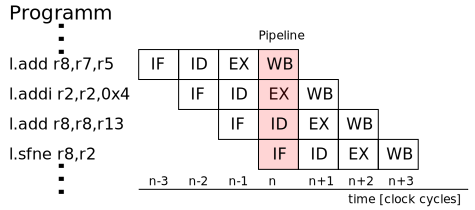
\includegraphics[scale=0.8]{./figures/pipeline}
  \caption{Sample program execution for a pipelined architecture w/o hazard suppression.}
  \label{fig:pipe1}
\end{figure}  


Figure \ref{fig:pipe1} and Table \ref{tab:pipe1} show the execution of a sample program and illustrates the concurrency of four instruction at time $n$ in the pipelined architecture. In each pipeline stage, there is one different instruction processed. The numbers in Figure \ref{fig:pipe1} correspond to the register and branch flag values at according cycles.
\begin{table}[htbp]
			\centering

\begin{minipage}[t]{0.45\textwidth}

 \caption[Sample Execution of the one-cycle architecture]{Register values for the \\one-cycle architecture \\}
 \label{tab:pipe0}
\centering\begin{tabular}{|l|r|r|r|r|r||r|} \hline
time & r2 & r5 & r7 & r8 & r13 & F\footnote{(Branch) Flag} \\ \hline
$n-1$ & 6 & 3 & 4 & 0 & 3 & 0 \\ \hline
$n$ & - &-& - &7& - & - \\ \hline
$n+1$ & 10 &-& - & - & -& - \\ \hline
$n+2$ & - &-& - & 10 & - & - \\ \hline
$n+3$ & - &-& - & - & - & 0 \\ \hline \hline
$end$ & 10 & 3 & 4 & 10 &3 &0 \\ \hline


\end{tabular}
\end{minipage}
			\begin{minipage}[t]{0.45\textwidth}

 \caption[Sample Execution of the pipelined arch. w/o hazard suppression]{Register values for the \\pipelined architecture\\without hazard suppression}
 \label{tab:pipe1}
\centering\begin{tabular}{|l|r|r|r|r|r||r|} \hline
time & r2 & r5 & r7 & r8 & r13 & F \\ \hline
$n-1$ & 6 & 3 & 4 & 0 & 3 & 0 \\ \hline
$n$ & - &-& - &-& - & - \\ \hline
$n+1$ & - &-& - & 7 & - & - \\ \hline
$n+2$ & 10 &-& - &-& - & -\\ \hline
$n+3$ & - &-& -&3& - & -\\ \hline
$n+4$ & - &-& - &-& - & 1 \\ \hline \hline
$end$ & 10 & 3 & 4 & 3 &3&1 \\ \hline

\end{tabular}
\end{minipage}\hfill			

\end{table}

Unfortunately, there is a data hazard in the pipelined architecture leading to errorneous behaviour. This can be seen if table \ref{tab:pipe1} was compared to \ref{tab:pipe0} where no dependecies exist, the hazard occurs due to the fact, that the result is written in the \glslink{wb}{WB} stage and accessible even one cycle later, but already needed in the \glslink{id}{ID} stage of the following instructions. The first possibility to get rid of this problem is to stall the piepline and wait until the required data is available. This version is exhibited on Figure \ref{fig:pipe2} and Table \ref{tab:pipe2}.


\begin{figure}[htbp]
  \centering
  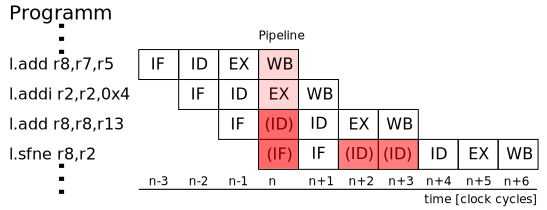
\includegraphics[scale=0.8]{./figures/pipeline2}
  \caption{Sample program execution for a pipelined architecture with stalls}
  \label{fig:pipe2}
\end{figure}

\begin{table}[htbp]
			\centering

\begin{minipage}[t]{0.45\textwidth}

 \caption[Sample Execution of the pipelined arch. with stalls]{Register values for the \\pipelined architecture\\ waiting for data}
 \label{tab:pipe2}
\centering\begin{tabular}{|l|r|r|r|r|r||r|} \hline
time & r2 & r5 & r7 & r8 & r13 & F \\ \hline
$n-1$ & 6 & 3 & 4 & 0 & 3 & 0 \\ \hline
$n$ & - &-& - &-& - & - \\ \hline
$n+1$ & - &-& - & 7 & - & - \\ \hline
$n+2$ & 10 &-& - &-& - & -\\ \hline
$n+3$ & - &-& -&-& - & -\\ \hline
$n+4$ & - &-& - &10& - & - \\ \hline 
$n+5$ & - &-& - &-& - & - \\ \hline 
$n+6$ & - &-& - &-& - & - \\ \hline 
$n+7$ & - &-& - &-& - & 0 \\ \hline \hline
$end$ & 10 & 3 & 4 & 10 &3&0 \\ \hline


\end{tabular}
\end{minipage}
			\begin{minipage}[t]{0.45\textwidth}

 \caption[Sample Execution of the pipelined arch. with forwarding]{Register values for the \\pipelined architecture\\with forwarding}
 \label{tab:pipe3}
\centering\begin{tabular}{|l|r|r|r|r|r||r|} \hline
time & r2 & r5 & r7 & r8 & r13 & F \\ \hline
$n-1$ & 6 & 3 & 4 & 0 & 3 & 0 \\ \hline
$n$ & - &-& - &-$\looparrowleft$& - & - \\ \hline
$n+1$ & - &-& - & $\looparrowright$7$\Uparrow$ & - & - \\ \hline
$n+2$ & 10 &-& - &$\uparrow$\ \ \ \ \ & - & -\\ \hline
$n+3$ & - &-& -&$\Uparrow$10\ \ & - & -\\ \hline
$n+4$ & - &-& - &-& - & 0 \\ \hline \hline
$end$ & 10 & 3 & 4 & 10 &3&0 \\ \hline

\end{tabular}
\end{minipage}\hfill			

\end{table}
\subsection{Forwarding}
A wide known technique to resolve this problem is forwarding. In this architecture variant register value A and/or B are replaced by the value calculated in the \glslink{ex}{EX} stage or aquired in the \glslink{wb}{WB} stage (e.g. data from data memory). A simplified forwarding block diagram is showed in fig TODO and the resulting execution of the sample program is showed in Figure \ref{fig:pipe3} and Table \ref{tab:pipe3}.

\begin{figure}[h!]
  \centering
  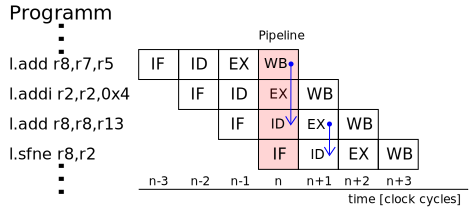
\includegraphics[scale=0.8]{./figures/pipeline3}
  \caption{Sample program execution for a pipelined architecture with forwarding}
  \label{fig:pipe3}
\end{figure}


\section{Controller}

Dividing the processor architecture into a data path and a control path is one of the keys to keep the source code and schemata readable. The data path takes care of all data and processes it, while the control path decides which route of the data path will be taken. In our case, we strictly separated the data path (Appendix~\ref{fig:cpu_schema}) from the control path, which we call the controller.

The main purpose of the controller is to decode the current instruction (Instruction Decode stage) and set all signals in order to route the operands to the correct destination. These signals include switching of the PC for jumps, selecting the correct ALU operation or multiplier mode (see Section~\ref{sec:multiplier}), enabling data write to the memory, setting required flags, etc.

Another quite important task of the controller is to detect hazards and to use forwarding or stalling in these cases accordingly. In most cases we tried to stall only where it was unavoidable and let operations run in parallel or forward data to prevent hazards.


\section{ALU}
The \gls{alu} is a substantial part of a processor. The ALU calculates all arithmetic operations needed by an instruction. Apart from the arithmetic operations, comparison and extension operations are as well executed to the ALU. The ALU needs four inputs: \textit{ALU\_Op\_DI} which indicates which operation has to be executed, the two 32 bits long operands \textit{Op1\_DI} and \textit{Op2\_DI}, and \textit{CY\_DI} - the carry bit\footnote{Carry bit is set if there was an unsigned overflow, e.g. $3'b101+3'b110=3'b011 \Rightarrow 5+6=3$} of the last executed l.add, l.addc or l.sub instructions. The outputs are the 32 bit long result \textit{Result\_DO}, the carry \textit{CY\_DO} and the overflow\footnote{Overflow bit is set if there was a signed overflow, e.g. $3'b011+3'b001=3'b100 \Rightarrow 3+1=-4$} \textit{OV\_DO}.

The ALU supports five different types of operations which are explained in the following sections.

\textbf{Adding Operations} \\
The first ones are the adding operations. These include addition with and without carry (input) and subtraction. Primarily we need a 32 bit full adder and an addition with and without carry. Secondary, the subtraction can be calculated by this adder if the subtrahend is two's complemented and used as second summand, this is realized by inverting each bit of the second operand and setting the carry input of the full adder to one.

Finally all these operations need to set or unset the carry and overflow flags in the \gls{spr}. The carry is already available from the full adder, it is the 33th bit of the result. Overflow may occur in two cases, the first one is a positive overflow when two positive numbers are added, but the result is negative and second one when two negative numbers are added and the result is positive. To check this the most significant bit of the operands and the result are compared. Figure \ref{fig:alu_add} shows the adder part of the ALU.

\begin{figure}[htbp]
  \centering
  \includegraphics[scale=0.95]{./figures/alu_add}
  \caption{ALU, adding operations.}
  \label{fig:alu_add}
\end{figure}

\textbf{Bitwise Operations} \\
Bitwise operations execute boolean operations on each bit. The in the ALU implemented bitwise operations are AND, OR and the exclusive or XOR\footnote{The boolean exclusive or operator returns 1 if the boolean inputs are not equal. e.g. for the bitwise XOR: 4'b0101 XOR 4'b1100 = 4'b1001} \\

\textbf{Shift Operations} \\
There are several shift operation which have to be supported. \\
- Shift Left Logical + MOVHI\\
- Shift Right Logical (unsigned) \\
- Shift Right Arithmetical (signed) \\
- Rotate Right Logical (Op1 << (32-Op2) | Op1 >> (32-Op2)) \\
\begin{figure}[htbp]
  \centering
  \includegraphics[scale=0.85]{./figures/alu_shift}
  \caption{ALU, shift operations.}
  \label{fig:alu_shift}
\end{figure}

\textbf{Extension Operations} \\
... \\

\textbf{Comparison Operations} \\
Siehe \ref{fig:alu_schema}


\section{Memory \& Wrapper}

As mentioned in Section~\ref{sec:top_design}, we have two memories namely an instruction memory and a data memory. Both are embedded in a wrapper in order to simplify the usage for the processor.

The actual memory modules used are 4 KB in size and have 32-bit inputs and outputs, where the inputs are byte-write enabled in order to work as intended with our CPU.

For the instruction memory, the access for the CPU is quite simple, because we always want to read the whole 32-bit word as our instruction. But we also want to be able to store a new program in the memory and because of our 8-bit interface, we need some input logic to write these bytes at the correct location.

In the data memory wrapper there is more to do, because the CPU needs the ability to store and load words, half-words and bytes. Last but not least we also want to be able to read out both, the data and the instruction memory and therefore, we need an 8-bit output interface, where this logic is already present for the data memory because of the load byte operation.


\section{Multiplier}
\label{sec:multiplier}

In order to perform calculations efficiently, we decided to do multiplications on a separate unit in parallel to the \gls{alu}. But because a 32-bit multiplication takes a long time compared to the other operations, we have to run it for more than one clock cycle. One design decision was therefore, how many cycles were optimal and how to implement this solution.

Our first attempt was to use FloPoCo\footnote{\url{http://flopoco.gforge.inria.fr}}, a generator of arithmetic cores (\textbf{Flo}ating-\textbf{Po}int \textbf{Co}res) which allowed us to generate \gls{vhdl} modules with the desired characteristics. But because FloPoCo is optimized for \glspl{fpga}, the results were not suitable for our project.

By now we figured out that two clock cycles should be enough for the multiplication to complete and we found two other possibilities how to achieve it: we could either use a DesignWare multiplier from Synopsys or try retiming of a standard multiplication. This works as follows: The multiplication is done as usual, but the result is not directly routed to the output, it is stored in a register. During the design compilation we then have the possibility to tell the compiler to take the whole multiplier and retime it, which means the register gets moved towards the middle of the multiplication, where we want it to be.\\
These were the results of the compilation for both possibilities with a clock period of 1.5~ns:

\begin{table}[htbp]
 \caption{Comparison of DesignWare vs. Retiming multiplier}
 \label{tab:designware}
 \centering
 
 \begin{tabular}{|l|r|r|}
  \hline
  & DesignWare & Retiming \\
  \hline
  Input $\to$ Register & 1.64 ns & 1.70 ns \\
  Register $\to$ Result & 1.21 ns & 1.16 ns \\
  Register $\to$ Overflow & 1.74 ns & 1.75 ns \\
  \hline
  Area & 133'713 $\mu m^2$ & 157'208 $\mu m^2$ \\
  \hline
 \end{tabular}
 
\end{table}

As we can see in Table~\ref{tab:designware}, the DesignWare multiplier is slightly faster than the retiming variant. But the difference is quite small and because we want to be as independent as possible, we decided to go with the retiming multiplier anyways.

\section{Stalls}
TBD
 \cleardoublepage
%%%%%%%%%%%%%%%%%%%%%%%%%%%%%%%%%%%%%%%%%%%%%%%%%%%%%%%%%%%%%%%%%%%%%%%
%%%%%%%%%%%%%%%%%%%%%%%%%%%%%%%%%%%%%%%%%%%%%%%%%%%%%%%%%%%%%%%%%%%%%%%
%%%%%                                                                 %
%%%%%     <file_name>.tex                                             %
%%%%%                                                                 %
%%%%% Author:      Renzo Andri                                        %
%%%%% Created:     21.12.2013                                         %
%%%%% Description: Chapter about Design Implementations and           %
%%%%%              Performance Data.                                  %
%%%%%                                                                 %
%%%%%%%%%%%%%%%%%%%%%%%%%%%%%%%%%%%%%%%%%%%%%%%%%%%%%%%%%%%%%%%%%%%%%%%
%%%%%%%%%%%%%%%%%%%%%%%%%%%%%%%%%%%%%%%%%%%%%%%%%%%%%%%%%%%%%%%%%%%%%%%


\chapter{Design Implementation}
\textit{This chapter is about the architecture variant you actually
implemented and its resulting performance; e.g., SNR, image quality,
peak throughput, required bandwidth ... (whatever quality and
performance metrics apply). In an ASIC or FPGA project you would also
specify the key figures of your design; e.g., area/lut usage, timing
figures, interface widths... In an ASIC project you would also talk
about backend specific things such as the floorplan of your chip,
design for test (and test coverage), power simulation, special
clocking circuitry and pad/bonding diagrams.}


\section{Instruction Table}
The following Table \ref{tab:instr} gives an overview of the implementented \gls{orbis} instructions. See Table \ref{tab:instr_det} for more detailled information about the functionality of each instruction and consider Table \ref{tab:conv} for naming conventions.
%\begin{landscape}
\begin{longtable}{|p{1.8cm}|l|p{10cm}|}
\caption[Instructions]{Instructions}

\label{tab:instr}
\endfirsthead
\multicolumn{3}{c}{Table \ref{tab:instr}: Instructions (contin.)} \\ \hline
Instruction & Parameter & Description \\ \hline
\endhead
\endfoot
\endlastfoot
\hline
Instruction & Parameter & Description \\ \hline
l.bf&N&Brach if Flag\\ \hline
l.bnf&N&Branch if not Flag\\ \hline
l.j&N&Jump Immediate\\ \hline
l.jal&N&Jump and Link\\ \hline \hline

l.nop&K&No Operation\\ \hline \hline

l.jalr&rB&Jump and Link Register\\ \hline
l.jr&rB&Jump Register\\ \hline \hline

l.movhi&rD, K&Move High\\ \hline
l.addi&rD, rA, I&Add Immediate\\ \hline
l.addic&rD, rA, I&Add Immediate Carry\\ \hline
l.andi&rD, rA, K&Bitwise And Immediate\\ \hline
l.lbs&rD, I(rA)&Load Byte Signed\\ \hline
l.lbz&rD, I(rA)&Load Byte Unsigned\\ \hline
l.lhs&rD, I(rA)&Load Halfword Signed\\ \hline
l.lhz&rD, I(rA)&Load Halfword Unsigned\\ \hline
l.lws&rD, I(rA)&Load Word Signed\\ \hline
l.lwz&rD, I(rA)&Load Word Unsigned\\ \hline
l.mfspr&rD, rA, K&Move from Special-Purpose Register\\ \hline
l.muli&rD, rA, I&Multiply Immediate\\ \hline
l.ori&rD, rA, K&Bitwise Or Immediate\\ \hline
l.xori&rD, rA, I&Bitwise Exclusive Or Immediate\\ \hline \hline

l.rori&rD, rA, L&Rotate Right Logic Immediate\\ \hline
l.slli&rD, rA, L&Shift Left Logic Immediate\\ \hline
l.srai&rD, rA, L&Shift Right Arithmetic Immediate\\ \hline
l.srli&rD, rA, L&Shift Right Logic Immediate\\ \hline \hline

l.mtspr&rA, rB, K&Move to Special-Purpose Register\\ \hline
l.sb&I(rA), rB&Store Byte\\ \hline
l.sh&I(rA), rB&Store Halfword\\ \hline
l.sw&I(rA), rB&Store Word\\ \hline \hline
 
l.add&rD, rA, rB&Add\\ \hline
l.addc&rD, rA, rB&Add Carry\\ \hline
l.and&rD, rA, rB&Bitwise And\\ \hline
l.or&rD, rA, rB&Bitwise Or\\ \hline
l.sll&rD, rA, rB&Shift Left Logic\\ \hline
l.sra&rD, rA, rB&Shift Right Arithmetic\\ \hline
l.srl&rD, rA, rB&Shift Right Logic\\ \hline
l.sub&rD, rA, rB&Subtract\\ \hline
l.xor&rD, rA, rB&Bitwise Exclusive Or\\ \hline
l.mul&rD, rA, rB&Multiply\\ \hline
l.mulu&rD, rA, rB&Multiply Unsigned\\ \hline
l.muld&rA, rB&Multiply Double-Word\\ \hline
l.muldu&rA, rB&Multiply Double-Word Unsigned\\ \hline \hline

l.sfeq&rA, rB&Set Flag if Equal\\ \hline
l.sfges&rA, rB&Set Flag if Greater Equal Signed\\  \hline
l.sfgeu&rA, rB&Set Flag if Greater Equal Unsigned\\ \hline
l.sfgts&rA, rB&Set Flag if Greater than Signed\\ \hline
l.sfgtu&rA, rB&Set Flag if Greater than Unsigned\\ \hline
l.sfles&rA, rB&Set Flag if Less Equal Signed\\ \hline
l.sfleu&rA, rB&Set Flag if Less Equal Unsigned\\ \hline
l.sflts&rA, rB&Set Flag if Less than Signed\\ \hline
l.sfltu&rA, rB&Set Flag if Less than Unsigned\\ \hline
l.sfne&rA, rB&Set Flag if not Equal\\ \hline \hline

l.sfeqi&rA, I&Set Flag if Equal Immediate\\ \hline
l.sfgesi&rA, I&Set Flag if Greater Equal Signed Immediate\\ \hline
l.sfgeui&rA, I&Set Flag if Greater Equal Unsigned Immediate\\ \hline
l.sfgtsi&rA, I&Set Flag if Greater than Signed Immediate\\ \hline
l.sfgtui&rA, I&Set Flag if Greater than Unsigned Immediate\\ \hline
l.sflesi&rA, I&Set Flag if Less Equal Signed Immediate\\ \hline
l.sfleui&rA, I&Set Flag if Less Equal Unsigned Immediate\\ \hline
l.sfltsi&rA, I&Set Flag if Less than Signed Immediate\\ \hline
l.sfltui&rA, I&Set Flag if Less thanb Unsigned Immediate\\ \hline
l.sfnei&rA, I&Set Flag if not Equal Signed Immediate\\ \hline \hline

l.extbs&rD, rA, rB&Extend Byte Signed\\ \hline
l.extbz&rD, rA, rB&Extend Byte Unsigned\\ \hline
l.exths&rD, rA, rB&Extend Half-Word Signed\\ \hline
l.exthz&rD, rA, rB&Extend Half-Word Unsigned\\ \hline
l.extws&rD, rA, rB&Extend Word Signed\\ \hline
l.extwz&rD, rA, rB&Extend Word Unsigned\\ \hline \hline

\multicolumn{2}{|l|}{l.eoc (cust1)}& Set "End of Computation" (Custom Instruction 1) \\ \hline

\end{longtable}

\section{Area}
\label{sec:area}
The colored Figure \ref{fig:chip_area} and Table \ref{tab:area_dist} give an overview of the occupied area. The multiplier is 19 \% of the required area, this is due to the fact that it is a multiplier with long operator sizes (33x33 signed) and the timing constraints are ambitious for only two pipeline stages. In fact it turned out that in the Sir10us project the multiplier is only about $74'000 \mu m^2$ in comparison to $159'000 \mu m^2$ only because the timing constraints are more lax.
\begin{figure}[htbp]
  \centering
  \includegraphics[width=\linewidth]{./figures/chip_colored}
  \caption{Area Distribution}
  \label{fig:chip_area}
\end{figure}

\begin{table}[htbp]
 \caption{Area distribution}
 \label{tab:area_dist}
 \centering\begin{tabular}{|l|r|r|r|r|r|} \hline
Name & Area [GE] & Cells & Area [$\mu m^2$] & $A/A_{tot}$ & Core Area \\ \hline
chip & 89174 & 15742 	& $1'607'457$ & 100.0 \% & - \\ \hline
-- pads and bondings 	& - &-&$771'501$ & - & - \\ \hline
-- top & 88592 & 15601 	& $830'497$ & 99.3 \% & 68.7 \%  \\ \hline
--- cpu & 44393 & 15218 & $416'160$ & 49.8 \% & 34.4 \%  \\ \hline
----- alu   & 5717 & 2283  	& $53'597$ & 6.4 \% & 4.4 \%\\ \hline
----- controller  & 482 & 273  	& $4'515$ & 0.6 \% & 0.4  \%\\ \hline
----- mult & 16930 & 6192 	& $158'709$ & 19.0 \% & 13.1 \% \\ \hline
----- registers& 13797 & 4037  	& $129'341$ & 15.5 \% & 10.7 \% \\ \hline
----- sp registers & 1133 & 267 & $10'621$ & 1.3 \% & 0.9 \% \\ \hline
--- instruction memory&21753& 58& $203'929$ & 24.4 \% & 16.9 \% \\ \hline
--- data memory  & 22260  & 257 & $208'676$ & 25.0 \% & 17.3 \% \\ \hline
 \end{tabular}
\end{table}
\newpage
\section{Timing}
As we have seen in chapter \ref{sec:pipe} - Pipelining is optimally used if the longest path of all pipeline stages are balanced. In table \ref{tab:longest_paths} there are listed all longest paths of the according four pipeline stages IF, ID, EX, WB and the two multiplier stages, a more detailled timinig diagram is shown in Figure \ref{fig:timing} where all paths between the pipeline stages is illustrated in an abstract way. The main stages are quite the same, but the Instruction Fetch stage is obviously quite shorter than the others. Combining with ID or WB seems not to be a feasible solution because they are already long enough and retiming could balance it but would lead to a less understandable design. 
\begin{table}[htbp]
 \caption{Longest Paths}
 \label{tab:longest_paths}
 \centering\begin{tabular}{|l|r|r|r|} \hline
\textbf{Pipeline Stage} & \textbf{$t_{pd}$} & \textbf{$t_{su}$} & \textbf{$\Sigma{t}$} \\ \hline
Instruction Fetch & 2.28 ns & 0.12 ns & 2.40 ns \\ \hline
Instruction Decode & 2.54 ns & 0.19 ns & 2.73 ns \\ \hline
Execute & 2.55 ns & 0.19 ns & 2.74 ns \\ \hline
- Execute ALU & 2.55 ns & 0.19 ns & 2.74 ns \\ \hline
- Execute Mult & 2.44 ns & 0.17 ns & 2.61 ns  \\ \hline
- Execute Mult 2 & 2.43 ns & 0.13 ns & 2.56 ns \\ \hline
Write Back & 2.55 ns & 0.19 ns & 2.74 ns \\ \hline \hline
Maximum & 2.59 ns & & 2.74 ns \\ \hline
Mean & 2.48 ns & & 2.63 ns\\ \hline
Standard Deviation & 0.15 ns & & 0.13 ns \\ \hline
 \end{tabular}
\end{table}

\begin{landscape}
\begin{figure}[htbp]
  \centering
  \includegraphics[width=\linewidth]{./figures/timing_diagram}
  \caption{Timing Diagram}
  \label{fig:timing}
\end{figure}

\end{landscape}

\section{Power}
Stichwort IR Drop, electromigration
\begin{table}[htbp]
 \caption{Power}
 \label{tab:power}
 \centering\begin{tabular}{|l|r|r|r||r||r|c|} \hline
program & $P_{SETUP}$ & $P_{RUN}$ & $P_{OUT}$ & $V_{cc_{min}}$ & $I_{max}$ & $\frac{J}{J_{max}}$ \\ \hline
full\_coverage.S & 53.9 $mW$ & 166.7 $mW$ & 64.8 $mW$ & 1.7943 $V$ & 6.97 $mA$ & 22 \% \\ \hline
matrixMul.c & 41.6 $mW$ & 161.2 $mW$ & - & 1.7905 $V$ & 11.42 $mA$ & 35 \% \\ \hline
matrixAdd.c & 43.5 $mW$ & 162.2 $mW$ & - & 1.7900 $V$ & 12.02 $mA$ & 37 \% \\ \hline
fibonacci.c & 44.5 $mW$ & 171.5 $mW$ & - & 1.7902 $V$ & 11.83 $mA$ & 35 \% \\ \hline \hline
mean/min/max & 45.9 $mW$ & 165.4 $mW$ & 64.8 $mW$ & 1.7900 $V$ & 12.02 $mA$ & 37 \%  \\ \hline
 \end{tabular}
\end{table}


\section{Floorplaning}
The floorplan is illustrated in Figure \ref{fig:chip_area}.
 \cleardoublepage
%%%%%%%%%%%%%%%%%%%%%%%%%%%%%%%%%%%%%%%%%%%%%%%%%%%%%%%%%%%%%%%%%%%%%%%
%%%%%%%%%%%%%%%%%%%%%%%%%%%%%%%%%%%%%%%%%%%%%%%%%%%%%%%%%%%%%%%%%%%%%%%
%%%%%                                                                 %
%%%%%     <file_name>.tex                                             %
%%%%%                                                                 %
%%%%% Author:      Renzo Andri                                        %
%%%%% Created:     30.11.2013                                         %
%%%%% Description: <description>                                      %
%%%%%                                                                 %
%%%%%%%%%%%%%%%%%%%%%%%%%%%%%%%%%%%%%%%%%%%%%%%%%%%%%%%%%%%%%%%%%%%%%%%
%%%%%%%%%%%%%%%%%%%%%%%%%%%%%%%%%%%%%%%%%%%%%%%%%%%%%%%%%%%%%%%%%%%%%%%



\chapter{Verification and Testing}
Testing is a substantial part in \gls{asic} design. In comparison to \gls{fpga} design, where faults can be corrected later, this is not possible on \glspl{asic} because wire and gate placement is fixed after tape-out. This leads to a right the first time policy and a high testing effort during all design stages. 
But also faults in production may lead to faulty chips. Therefore, all procuded chips have to be tested efficiently to detect as many as possible of these faulty chips to avoid selling these faulty chips. \cite{vlsi3}

\section{Testbench and Testing interface}
In an usual test setup, there is a stimuli application interface and after or during execution responses are read and compared to expected responses. \cite{vlsi1} This testing scheme was an inspiration for our one, but could not have been adapted directly because a processor behaves in an other way. The used test scheme is illustrated in Figure \ref{fig:testbenchSchema} and in the following sections.

\subsection{Stimuli application, SETUP mode}
In the SETUP mode instructions and data have to be loaded into the instruction and data memory, respectively. Therefore a stimuli file is read. Each stimuli entry consists of the byte address (first 13 bits\footnote{This number depends on the memory size. In the OR10N chip there are 8'192 bytes addressable, therefore address length has to be chosen as $l_{adr}=13=\log_2 8192$}) and one word (32 bit instruction/ 32 bit data). Due to the small number of pins the data is then applied bytewise with the according byte address. See Ch. \ref{sec:mem_addr} for more information about memory addressing.

\begin{landscape}
\begin{figure}[t!]

\centering
\includegraphics[scale=0.8]{figures/tb3.pdf}
\caption{Schema of the testbench}
\label{fig:testbenchSchema}
\end{figure}
\end{landscape}

\subsection{RUN mode}
In RUN mode the cpu is enabled and the testbench waits on the end of computation signal. During running the testbench applies the acknowledgement signal for the data and the instruction memory to simulate the behaviour of the processor in a multi-core system. This can be either from file or by random generator. See appendix \ref{chapt:files} for more information how to use the testbench.

\subsection{Response Acquisition, READOUT mode}
The third mode checks whether the memory entries are as expected. For this reason a response file is read. Like in the SETUP mode the entries consist of the byte address (pointing to the MSB byte of the word) and the data word. Each byte address of the required word is then applied separately and the data can be read from the the \textit{Data\_DIO} output one cycle later and put together to compare the expected word.


\section{Functional Verification}
Functional verification is done with a few chips (prototypes) to check if the chips behave as expected. This includes in the ideal case the testing of the whole set of functionality and states of the chip. Faults detected in this design stage can have already a high economic impact because all chips behave in a wrong way. Therefore verification by simulation before tape-out is very important.

\subsection{Verification by simulation}
The simulation tool used in this thesis is ModelSim of MentorGraphics. Simulation allows us to check the chip functionality during early design steps but also provides the possibility to check if generated stimuli vectors have a high coverage in chip functionality. These stimuli with high coverage are later used to test chips after tape-out. In this thesis we used two possibilities to guarantee a high coverage: Code coverage and covergroups. \\\\
\textbf{Code coverage}
is a feature of ModelSim which counts during simulation how often every line was executed and which branches were taken. It takes also into consideration whether signals had toggled during simulation. By means of this we developed the programm \textit{full\_coverage} which can be found in the directory \textit{/sw/testscripts/full\_coverage.s}. Table \ref{tab:code_coverage} shows the coverage of this Assembler program. The relative bad Code Coverage for the top entity arises mainly by the fact that higher address bits (instruction and data memory) have never toggled. This is because we used only 4 kBit memory which can fully be addressed with 12 bits, these signals are cleaned out during synthesis anyway. \\
\begin{table}[htbp]
 \caption{Code coverage of the programm \textit{full\_coverage.S}}
 \label{tab:code_coverage}
 \centering\begin{tabular}{l l l r} \toprule
\multicolumn{3}{l}{\textbf{Module}} & \textbf{Coverage} \\ \midrule
\multicolumn{3}{l}{| Top} & \textbf{89.1 \%} \\
\  & \multicolumn{2}{l}{| CPU} & 96.3 \% \\
\ & \ & | ALU & 100.0 \% \\
\ & \ & | Multiplier & 99.9 \% \\
\ & \ & | Special-Purpose Register & 94.5 \% \\
\ & \ & | Registers & 99.7 \% \\
\ & \multicolumn{2}{l}{| Data Memory} & 92.0 \% \\
\  & \multicolumn{2}{l}{| Instruction Memory} & 96.3 \% \\ \bottomrule
 \end{tabular}
\end{table}
\\\\
\textbf{Covergroups:}
Code coverage does already give a good insight in coverage but lacks the opportunity to check whether special critical cases occurr concurrently. Therefore we expanded our coverage analysis with so-called covergroups. Covergroup is a special class which is provided by SystemVerilog but not by \gls{vhdl}. This class allows to select signals the simulator has to listen for, and to define bins containing signal values which belong together. \cite{SVG} During simulation runs with enabled coverage option\footnote{To run ModelSim in coverage mode add \textit{-coverage} to \textit{vsim}. More detailled explanation on how to simulate the processor can be found in appendix \ref{chapt:files}.}, ModelSim counts how often a signal matches the values defined in the bins and monitors them.
Table \ref{tab:covergroups} shows the covergroups defined for coverage analysis for this thesis and Figure \ref{fig:cov_over} shows the resulting coverage analysis for the \textit{full\underline{ }coverage} program.

\begin{table}[htbp]
 \caption{Covergroups}
 \label{tab:covergroups}
 \centering\begin{tabular}{l l p{8cm}} \hline
Covergroup & Coverpoint & Goal: Coverage of ... \\ \hline
Instructions& Types & all instruction types. (R-, I-, J-type, ...) \\
 & Jump & all different jump instructions. (l.j, l.bf, ...) \\
 & Load & all different load instructions. (l.lws, l.lbz, ...)\\
 & Store & all differnet store instructions. (l.sw, l.sh, l.sb) \\
 & Immediate & all different immediate instructions. (l.addi, l.movhi, l.ori, ...) \\
 & R-type & ALU and Shift operations. (l.add, l.sll, ...). \\
 & SPR & move to/from Special-Purpose register. \\
 & Others & all other instructions. (l.nop, l.eoc) \\ \hline
ALU & ALU\underline{ }Op & all ALU operations \\ 
 & CY\underline{ }Set & at least one (unsigned) carry overflow. \\
  & OV\underline{ }Set & at least one signed overflow. \\
  & CompareNFlag & at least one SetFlag to 0 and 1. \\
  & *\underline{ }Set\underline{ }CY & carry overflow for l.add, l.addc and l.sub. \\
  & *\underline{ }Set\underline{ }OV & signed overflow/underflow for l.add, l.addc and l.sub. \\ \hline
Mult & DoubleWord & at least one double word multiplication. \\ 
 & Mult\underline{ }CY & at least one carry overflow multiplication. \\
 & Mult\underline{ }OV & at least one signed overflow multiplication. \\
 & Mult\underline{ }Stage1n2 & at least one multiplication in both stages.\\
 & Mult\underline{ }ALU\underline{ }Conc & at least one multiplication and \gls{alu} Operation concurrently. \\ \hline
 Stall & lw\underline{ }Stall & at least one stall due to dependency between load word data and data needed for subsequent instruction. \\ 
  & CacheMiss & at leat one stall due to a cache miss (data memory). \\
  & InstrMiss & at least one stall due to a cache miss (instruction memory). \\
  & MultStall & at least one stall due to a multiplication. \\ \hline
Forward & EX2ID & at least one data dependency between EX and ID stage. \\ 
 & WB2ID & at least one data dependency between WB and ID stage. \\
 & EX2IDnWB & at least one data dependency between WB, EX and ID stage.
\\ \hline
 \end{tabular}
\end{table}

\begin{figure}[tb]
  \centering
  \includegraphics[width=\linewidth]{./figures/covergroups_overview.png}
  \caption{Covergroups for \textit{full\underline{ }coverage} in Modelsim}
  \label{fig:cov_over}
\end{figure}


\textbf{C programs}: 
Although it is possible to write good Assembler codes, it is hard to write complex programs. OpenCores Community provides a C C compiler which allows to translate C programs into Assembly. This allows us to write programs in the high level language C and generate Assembler code which can then ceasily be translated into machine code. Generating expected responses is simplified because such programs can be compiled and run on a Golden Model (computer's cpu). See appendix \ref{chapt:files} for more information.

\section{Production test}
As mentioned in the introduction to this chapter production faults can play a decisive role. The yield\footnote{Yield defines the ratio of error-free chip to produced chips.} deviates mainly depending on circuit complexity and integration scale. Therefore, errornous chips have to be detected before selling. All produced chips have to be checked in reasonable time and all faulty chips should be rejected. There are several good possibilities to guarantee a high fault detection rate, the used \gls{dft} approaches are mentioned in the following lines.

\subsection{Scan Chain}
High testability needs a high controllability and high observability of as many nodes as possible. If internal complexity rises, these criteria cannot be fullfilled any more due to the lack of (output) pins. In this thesis, 1'712 flip-flops and 84 k\glslink{ge}{GE} are used but only 46 pins are available at all. Therefore, all flip-flops are replaced with scan flip-flops. A scan flip-flop has two additional singals: an enable signal (\textit{Test\underline{ }En\underline{ }TI}) and a scan input signal. Synopsys then connects these Scan-FF to a shift register. To set up the FF to the test vectors' values, data can be passed through the whole scan chain. The scan enable signal can be driven to low and one clock period later all flip-flops have settled and can be read out the other way round using the scan chain. \\

\begin{table}[htbp]
 \caption{Scan Chains}
 \label{tab:scan_chain}
 \centering\begin{tabular}{|l|r|} \hline
Scan Chain 1-2 & 172 \\ \hline
Scan Chain 3-10 & 171 \\ \hline
Non-Scan-FF & 0 \\ \hline
Total & 1'712 \\ \hline
 \end{tabular}
\end{table}


\subsection{Automated Test Pattern Generation (ATPG)}
To get reasonable test vectors we use ATPG supported by Tetramax. First Tetramax builds a so-called fault dictionary where all possible detectable stuck-at\footnote{Stuck-at faults depend to a fault model where production faults causes the node to keep some value although it may be driven to some other value.\cite{vlsi3}} faults are collected. With this dictionary Tetramax is able to generate a test pattern which can be used with the available scan chains to detect possible flaws. 




\subsection{Testing the Reset signal}
Stuck-at-one (s-a-1) fault somewhere in the (active-low) Reset signal tree can't be detected by the scan chain because the reset signal is not part of the chain. To get rid of these (ATPG) undetectable faults, we will use the reset signal to set all registers to their initial values and read out these values using the chains. Table \ref{tab:fault_coverage} illustrates the consequent fault coverage.

%\subsection{Block isolation}

\begin{table}[htbp]
 \caption{Fault coverage with Scan-Chains using ATPG}
 \label{tab:fault_coverage}
 \centering\begin{tabular}{|l|r|} \hline
\textbf{fault class} & \textbf{faults} \\ \hline\hline
Detected & 99'448 \\ \hline
Detected (Rst/s-a-1) & 1'712 \\ \hline
Possibly detected & 116 \\ \hline
Undetectable & 321 \\ \hline
ATPG untestable & 1'312 \\ \hline
Not detected & 2 \\ \hline \hline
total faults & 102'910 \\ \hline
\textbf{test coverage} & \textbf{98.30 \%} \\ \hline
 \end{tabular}
\end{table}

TetraMAX determined 102'910 nodes which could be affacted by a stuck-at faults. With ATPG TetraMAX was able to generate patterns such that 99'448 of these stuck-at faults are detectable, additional 1'712 are detectable with the initial sequence. The Defect Level (DF)\footnote{The Defect Level ratioes the defective sold chips to all sold chips and can be approximated by the formula $DL=1-Y^{1-T}$ where Y is the yield and T the test coverage.\cite{vlsi3}} is 0.18 \% if a yield of 90 \% is assumed.

\subsection{Testing the memories}
The test coverages of the memories are low and it is not possible to improve this directly. Observability and controllability of the combinatoric circuits which connect the memories with the CPU cannot be fully realized, although a special bypass\footnote{Inspired by block isolation, we bypassed the memories in Test mode such that the memory wrapper can be tested without being able to check the memories by ATPG directly. Consider schemata in appendix \ref{ch:schemata} of the instruction and data memory.} was designed. For this reason the memories are fully accessible (read/write) from outside during setup mode. Memory testing will then be done with well-known methods like walking-zeros or walking-ones. 



 \cleardoublepage
%%%%%%%%%%%%%%%%%%%%%%%%%%%%%%%%%%%%%%%%%%%%%%%%%%%%%%%%%%%%%%%%%%%%%%%
%%%%%%%%%%%%%%%%%%%%%%%%%%%%%%%%%%%%%%%%%%%%%%%%%%%%%%%%%%%%%%%%%%%%%%%
%%%%%                                                                 %
%%%%%     07_results.tex                                              %
%%%%%                                                                 %
%%%%% Author:      <Renzo Andri>                                      %
%%%%% Created:     <Dec 14, 2013>                                     %
%%%%% Description: ...                                                %
%%%%%                                                                 %
%%%%%%%%%%%%%%%%%%%%%%%%%%%%%%%%%%%%%%%%%%%%%%%%%%%%%%%%%%%%%%%%%%%%%%%
%%%%%%%%%%%%%%%%%%%%%%%%%%%%%%%%%%%%%%%%%%%%%%%%%%%%%%%%%%%%%%%%%%%%%%%

\chapter{Results}
The goal of this thesis was a redesign of the already existing OpenRISC implementation\cite{website:OpenCores}. This implementation will be called \textit{"original"} in the following chapter. The original implementation has already been optimized and will be refered as the \textit{"optimized"} implementation. Both of these implementations were synthesized with the same setup as our implementation to guarantee for comparable data.
\section{Throughput Comparison}
To compare different processor architectures different performance measures can be used. When comparing different processors the frequency can be compared. This criteria is highly dependent on the number of pipeline stages and does not consider how many and which instruction was executed in each cycle.
Therefore, the first performance measure we used is \gls{ipc} which ratioes the number of effective executed instructions to the number of cycles needed to execute them. An optimal \gls{ipc} in a single-cycle RISC architecture would be 1, but this value cannot be reached by a pipelined architecture because at the end all final instructions have to pass all pipeline stages: With four stages as we used, there are always three additional cycles to finish execution. "No operation" (l.nop) which are usually injected by compiler\footnote{An example why the OpenRISC compiler reasonably adds a l.nop is the delay slot after a jump instruction. The instruction which follows a jump instruction is executed in the so-called delay slot, usually the compiler tries to reorder the operations such that an expendient instruction is put into the delay slot. If this was not possible due to some dependency, the compiler adds a l.nop instead.} are not counted as effective executed instructions and decrease IPC. The main source of a decreased IPC are stalls. Equations \ref{equ:ipc}\footnote{$\mathbbm{1}$ stands for the indicator function: $\mathbbm{1}_{condition}=\begin{cases}
								1 & \text{condition fullfilled},\\
								0 & \text{else}.
							    \end{cases}$} and \ref{equ:ipc2} show a formal description of the used IPC calculation.
\begin{equation}
\label{equ:ipc} 
IPC=\frac{\#instructions}{\#cycles}=\frac{\sum_{k=k_{start}}^{k_{end}} \mathbbm{1}_{(Instr[k]\ne'nop' \wedge PC[k]\ne PC[k-1])}}{3+(k_{end}-k_{start}+1)}
\end{equation}
\begin{equation}
\label{equ:ipc2} 
IPC=\frac{\#instructions}{\#cycles}=\frac{(k_{end}-k_{start}+1)-\#nop-\#stalls}{3+(k_{end}-k_{start}+1)} 
\end{equation}

Table \ref{tab:ipc} shows \gls{ipc} values of OR10N for seven sample programs and Table \ref{tab:ipc_comp} compares the resulting \gls{ipc} with them from the original and optimized implementation. The sample programs were chosen such that all kinds of operations are covered: These are branch, computation and storage intensive functions.
\begin{table}[htbp]
 \caption{IPC for sample programs on OR10N}
 \label{tab:ipc}
\centering\begin{tabular}{|l|r|r|r|r|r|} \hline
program name & \#instr. & \#nop & \#stalls & \#cycles & \gls{ipc} \\ \hline
fullCoverage.S   & 336  & 31 &    20 &    390 & 0.8615 \\ \hline
matrixMul.c    & 5'537  & 10 &   512 &  6'062 & 0.9134 \\ \hline
matrixAdd.c    & 5'341  & 15 &     0 &  5'359 & 0.9966 \\ \hline
stencil.c      & 1'656  & 44 &   111 &  1'814 & 0.9129 \\ \hline
towerofHanoi.c& 88'209  & 56 & 2'048 & 90'316 & 0.9767 \\ \hline
fibonacci.c    & 3'536 & 223 &    10 &  3'772 & 0.9374 \\ \hline
bubblesort.c &  70'704 & 101 & 4'950 & 75'758 & 0.9333 \\ \hline
\end{tabular}
\end{table}


\begin{table}[htbp]
 \caption{Comparison of IPC}
 \label{tab:ipc_comp}
\centering\begin{tabular}{|l|r|r|r||r|r|} \hline
program & original & optimized & OR10N & \multicolumn{2}{c|}{Improvement} \\ \cline{1-4} \cline{5-6}
matrixMul.c & 0.5458 & 0.9996 & 0.9134 & +83.14\% & +67.35\% \\ \hline
matrixAdd.c & 0.6697 & 0.9960 & 0.9966 & +48.72\% & +48.81\% \\ \hline
stencil.c & 0.6095 & 0.9572 & 0.9129 & +57.05\% & +49.78\% \\ \hline
towerofHanoi.c & 0.6143 & 0.9773 & 0.9767 & +59.09\% & +58.99\% \\ \hline
fibonacci.c & 0.5695 & 0.9101 & 0.9374 & +59.81\% & +64.60\% \\ \hline
bubblesort.c & 0.6484 & 0.9329 & 0.9333 & +43.88\% & +43.94\% \\ \hline\hline
Mean \o & 0.6095 & 0.9622 & 0.9451 & +57.86\% & +55.04\% \\ \hline
\end{tabular}
\end{table}

As expected the optimized and our implementation are 57 \% and 55 \% better than the original one. The main reasons are the longer latency of the multiplication, which lasts four cycles in the original implementation instead of two, which results in more stalls than in the optimized and in our implementation. The comparison between our implementation and the optimized shows some benefit for the optimized implementation. Mainly because multiplications can be more efficiently executed due to aditional write ports at the \gls{gpr}. This increases the area and setup delay of the \gls{gpr}.  \\ \\

An even better performance measure is \gls{ops}, or \gls{mops} which indicates how many effective executed instructions are executed in one second. This measure can easily be determined with \gls{ipc} and the maximal clock frequency. Equation \ref{equ:ops} and \ref{equ:mops} shows this relation. 

\begin{equation}
\label{equ:ops}
\Theta_{OPS} = IPC \cdot f_{clk}= \frac{IPC}{T_{clk}}
\end{equation}
\begin{equation}
\label{equ:mops}
\Theta_{MOPS} = \Theta_{OPS} \cdot \left( \frac{10^{-6}\ MOPS}{1\ OPS}\right)
\end{equation}

Table \ref{tab:ops_cmp} and diagram \ref{fig:results} compare the throughput in \gls{mops} of the three implementations of the sample programs. The white part of the bars indicates the difference of the actual \gls{ipc} to an optimal IPC of 1. The original architecture is shown in red, the optimized one in blue and the OR10N architecture in green.

\begin{table}[htbp]
 \caption{Throughput comparison in MOPS}
 \label{tab:ops_cmp}
\centering\begin{tabular}{|l|r|r|r||r|r|} \hline
program & original & optimized & OR10N & \multicolumn{2}{c|}{Improvement} \\ \hline
matrixMul.c & 184.39 & 305.69 & 333.36 & +65.78\% & +80.79\% \\ \hline
matrixAdd.c & 226.25 & 304.59 & 363.72 & +34.62\% & +60.76\% \\ \hline
stencil.c & 205.91 & 292.72 & 333.18 & +42.16\% & +61.80\% \\ \hline
towerofHanoi.c & 207.53 & 298.87 & 356.46 & +44.01\% & +71.76\% \\ \hline
fibonacci.c & 192.40 & 278.32 & 342.12 & +44.66\% & +77.82\% \\ \hline
bubblesort.c & 219.05 & 285.29 & 340.62 & +30.24\% & +55.50\% \\ \hline\hline
Mean \o & 205.92 & 294.25 & 344.91 & +42.89\% & +67.49\% \\ \hline
\end{tabular}
\end{table}

Due to the higher maximal frequency of the proposed implementation, an even higher throughput is achieved compared to the original implementation. OR10N achieves 17 \% higher throughput than the optimized implemenation because of the shorter longest path, a comparison of the maximal frequencies and areas are showed in Table \ref{tab:area_cmp}. Section \ref{sec:area} shows detailed information about the area distribution of OR10N.

\begin{figure}[t!]
\centering
%\includepdf{figures/instr_mem.pdf}
\includegraphics[scale=0.6]{figures/results.png}
\caption{Comparison between OR10N, original and optimized architecture. TODO: replace!!}
\label{fig:results}

\end{figure}

\begin{table}[htbp]
 \caption{Area and frequency comparison}
 \label{tab:area_cmp}
\centering\begin{tabular}{|r|r|r||r|r|} \hline
implementation & \multicolumn{2}{c||}{area} & \multicolumn{2}{c|}{$f_{max}$} \\ \hline
original & 755'608 $\mu m^2$ & $-$ & 337.84 MHz & $-$ \\ \hline
optimized & 789'090 $\mu m^2$ & $+$4.43 \% & 305.81 MHz & $-$9.48 \% \\ \hline
OR10N & 779'200 $\mu m^2$ & $+$3.12 \% & 364.96 MHz & $+$8.03 \% \\ \hline
\end{tabular}
\end{table}




 \cleardoublepage
%%%%%%%%%%%%%%%%%%%%%%%%%%%%%%%%%%%%%%%%%%%%%%%%%%%%%%%%%%%%%%%%%%%%%%%
%%%%%%%%%%%%%%%%%%%%%%%%%%%%%%%%%%%%%%%%%%%%%%%%%%%%%%%%%%%%%%%%%%%%%%%
%%%%%                                                                 %
%%%%%     <file_name>.tex                                             %
%%%%%                                                                 %
%%%%% Author:      <author>                                           %
%%%%% Created:     <date>                                             %
%%%%% Description: <description>                                      %
%%%%%                                                                 %
%%%%%%%%%%%%%%%%%%%%%%%%%%%%%%%%%%%%%%%%%%%%%%%%%%%%%%%%%%%%%%%%%%%%%%%
%%%%%%%%%%%%%%%%%%%%%%%%%%%%%%%%%%%%%%%%%%%%%%%%%%%%%%%%%%%%%%%%%%%%%%%

\chapter{SystemVerilog vs. VHDL}
Eventuell noch ein SystemVerilog chapter



 \cleardoublepage
\include{./content/08_conclusion} \cleardoublepage


%%%%%
%%%%% Start of additional parts.
%%%%%
\appendix

%%%%%%%%%%%%%%%%%%%%%%%%%%%%%%%%%%%%%%%%%%%%%%%%%%%%%%%%%%%%%%%%%%%%%%%
%%%%%%%%%%%%%%%%%%%%%%%%%%%%%%%%%%%%%%%%%%%%%%%%%%%%%%%%%%%%%%%%%%%%%%%
%%%%%                                                                 %
%%%%%     <file_name>.tex                                             %
%%%%%                                                                 %
%%%%% Author:      <author>                                           %
%%%%% Created:     <date>                                             %
%%%%% Description: <description>                                      %
%%%%%                                                                 %
%%%%%%%%%%%%%%%%%%%%%%%%%%%%%%%%%%%%%%%%%%%%%%%%%%%%%%%%%%%%%%%%%%%%%%%
%%%%%%%%%%%%%%%%%%%%%%%%%%%%%%%%%%%%%%%%%%%%%%%%%%%%%%%%%%%%%%%%%%%%%%%


\chapter{Declaration of Originality}\label{chap:originality}
% include the signed declaration of authorship!
\includepdf[pages=-, turn=false, scale=0.9]{./figures/declaration_of_originality}

 \clearpage
%%%%%%%%%%%%%%%%%%%%%%%%%%%%%%%%%%%%%%%%%%%%%%%%%%%%%%%%%%%%%%%%%%%%%%%
%%%%%%%%%%%%%%%%%%%%%%%%%%%%%%%%%%%%%%%%%%%%%%%%%%%%%%%%%%%%%%%%%%%%%%%
%%%%%                                                                 %
%%%%%     <file_name>.tex                                             %
%%%%%                                                                 %
%%%%% Author:      <author>                                           %
%%%%% Created:     <date>                                             %
%%%%% Description: <description>                                      %
%%%%%                                                                 %
%%%%%%%%%%%%%%%%%%%%%%%%%%%%%%%%%%%%%%%%%%%%%%%%%%%%%%%%%%%%%%%%%%%%%%%
%%%%%%%%%%%%%%%%%%%%%%%%%%%%%%%%%%%%%%%%%%%%%%%%%%%%%%%%%%%%%%%%%%%%%%%

\chapter{Instructions}
Table \ref{tab:instr_det} complements table \ref{tab:instr} with a more detailled description about the functionality of the instruction set. Instruction description and naming conventions are adopted from the OpenRISC 1000 Architecture Manual and are explained in table \ref{tab:instr_conv}.
\begin{table}[htbp]
 \caption{Naming conventions}
 \label{tab:instr_conv}
 \centering\begin{tabular}{|c|l|} \hline
l.* & \gls{orbis} instruction \\ \hline

l.*s & The result of this instruction is sign-extended (exts). \\ \hline
l.*z & The result of this instruction is zero-extended (extz). \\ \hline
rX & General-Purpose Register X \\ \hline
SR & Supervision Register \\ \hline
spr & Special-Purpose Register \\ \hline
K & Immediate Operand is zero-extended. \\ \hline
I & Immediate Operand is sign-extended. \\ \hline
L & Length Immediate (zero-extended) \\ \hline
X & Don't Care Bits in Instruction Encoding \\ \hline
[*] & Address space \\ \hline
(*) & Memory entry at specified address \\ \hline
\{*\} & Operations in brackets are executed prior assignment. \\ \hline

 \end{tabular}
\end{table}

\begin{longtable}{|p{3cm}|p{10cm}|}
\caption[Instructions detailed]{Instructions detailed}
\label{tab:instr_det}
\endfirsthead
\multicolumn{2}{c}{Table \ref{tab:instr_det}: Instructions detailed (contin.)} \\
\endhead
\endfoot
\endlastfoot
\hline
l.add rD,rA,rB & rD[31:0] $\leftarrow$ rA[31:0] + rB[31:0]\newline SR[CY] $\leftarrow$ carry\newline SR[OV] $\leftarrow$ overflow \\ \hline
l.addc rD,rA,rB & rD[31:0] $\leftarrow$ rA[31:0] + rB[31:0] + SR[CY]\newline SR[CY] $\leftarrow$ carry\newline SR[OV] $\leftarrow$ overflow \\ \hline l.addi rD,rA,I & rD[31:0] $\leftarrow$ rA[31:0] + exts(Immediate)\newline SR[CY] $\leftarrow$ carry\newline SR[OV] $\leftarrow$ overflow \\ \hline l.addic rD,rA,I & rD[31:0] $\leftarrow$ rA[31:0] + exts(Immediate) + SR[CY]\newline SR[CY] $\leftarrow$ carry\newline SR[OV] $\leftarrow$ overflow \\ \hline l.and rD,rA,rB & rD[31:0] $\leftarrow$ rA[31:0] AND rB[31:0] \\ \hline l.andi rD,rA,K & rD[31:0] $\leftarrow$ rA[31:0] AND extz(Immediate) \\ \hline l.bf N & EA $\leftarrow$ exts(Immediate $<<$ 2) + BranchInsnAddr\newline PC $\leftarrow$ EA if SR[F] set \\ \hline l.bnf N & EA $\leftarrow$ exts(Immediate $<<$ 2) + BranchInsnAddr\newline PC $\leftarrow$ EA if SR[F] cleared \\ \hline l.eoc=l.cust1  & EOC $\leftarrow$ 1 \\ \hline l.extbs rD,rA & rD[31:8] $\leftarrow$ rA[7]\newline rD[7:0] $\leftarrow$ rA[7:0] \\ \hline l.extbz rD,rA & rD[31:8] $\leftarrow$ 0\newline rD[7:0] $\leftarrow$ rA[7:0] \\ \hline l.exths rD,rA & rD[31:16] $\leftarrow$ rA[15]\newline rD[15:0] $\leftarrow$ rA[15:0] \\ \hline l.exthz rD,rA & rD[31:16] $\leftarrow$ 0\newline rD[15:0] $\leftarrow$ rA[15:0] \\ \hline l.extws rD,rA & rD[31:0] $\leftarrow$ rA[31:0] \\ \hline l.extwz rD,rA & rD[31:0] $\leftarrow$ rA[31:0] \\ \hline l.j N & PC $\leftarrow$ exts(Immediate $<<$ 2) + JumpInsnAddr \\ \hline l.jal N & PC $\leftarrow$ exts(Immediate $<<$ 2) + JumpInsnAddr\newline LR $\leftarrow$ DelayInsnAddr + 4 \\ \hline l.jalr rB & PC $\leftarrow$ rB\newline LR $\leftarrow$ DelayInsnAddr + 4 \\ \hline l.jr rB & PC $\leftarrow$ rB \\ \hline l.lbs rD,I(rA) & EA $\leftarrow$ exts(Immediate) + rA[31:0]\newline rD[7:0] $\leftarrow$ (EA)[7:0]\newline rD[31:8] $\leftarrow$ (EA)[7] \\ \hline l.lbz rD,I(rA) & EA $\leftarrow$ exts(Immediate) + rA[31:0]\newline rD[7:0] $\leftarrow$ (EA)[7:0]\newline rD[31:8] $\leftarrow$ 0 \\ \hline l.lhs rD,I(rA) & EA $\leftarrow$ exts(Immediate) + rA[31:0]\newline rD[15:0] $\leftarrow$ (EA)[15:0]\newline rD[31:16] $\leftarrow$ (EA)[15] \\ \hline l.lhz rD,I(rA) & EA $\leftarrow$ exts(Immediate) + rA[31:0]\newline rD[15:0] $\leftarrow$ (EA)[15:0]\newline rD[31:16] $\leftarrow$ 0 \\ \hline l.lws rD,I(rA) & EA $\leftarrow$ exts(Immediate) + rA[31:0]\newline rD[31:0] $\leftarrow$ (EA)[31:0] \\ \hline l.lwz rD,I(rA) & EA $\leftarrow$ exts(Immediate) + rA[31:0]\newline rD[31:0] $\leftarrow$ (EA)[31:0] \\ \hline l.mfspr rD,rA,K & rD[31:0] $\leftarrow$ spr(rA OR Immediate) \\ \hline l.movhi rD,K & rD[31:0] $\leftarrow$ extz(Immediate) $<<$ 16 \\ \hline l.mtspr rA,rB,K & spr(rA OR Immediate) $\leftarrow$ rB[31:0] \\ \hline l.mul rD,rA,rB & rD[31:0] $\leftarrow$ rA[31:0] * rB[31:0]\newline SR[OV] $\leftarrow$ overflow\newline SR[CY] $\leftarrow$ carry \\ \hline
l.muld rA, rB & MACHI $\leftarrow$ \{rA[31:0] * rB[31:0]\}[63:32] \newline MACLO $\leftarrow$ \{rA[31:0] * rB[31:0]\}[31:0]\\ \hline
l.muldu rA, rB & MACHI $\leftarrow$ \{rA[31:0] * rB[31:0]\}[63:32] \newline MACLO $\leftarrow$ \{rA[31:0] * rB[31:0]\}[31:0]\\ \hline
   l.muli rD,rA,I & rD[31:0] $\leftarrow$ rA[31:0] * Immediate\newline SR[OV] $\leftarrow$ overflow\newline SR[CY] $\leftarrow$ carry \\ \hline l.mulu rD,rA,rB & rD[31:0] $\leftarrow$ rA[31:0] * rB[31:0]\newline SR[OV] $\leftarrow$ overflow\newline SR[CY] $\leftarrow$ carry \\ \hline l.nop K & \\ \hline l.or rD,rA,rB & rD[31:0] $\leftarrow$ rA[31:0] OR rB[31:0] \\ \hline l.ori rD,rA,K & rD[31:0] $\leftarrow$ rA[31:0] OR extz(Immediate) \\ \hline l.rori rD,rA,L & rD[31-L:0] $\leftarrow$ rA[31:L]\newline rD[31:32-L] $\leftarrow$ rA[L-1:0] \\ \hline l.sb I(rA),rB & EA $\leftarrow$ exts(Immediate) + rA[31:0]\newline (EA)[7:0] $\leftarrow$ rB[7:0] \\ \hline l.sfeq rA,rB & SR[F] $\leftarrow$ rA[31:0] == rB[31:0] \\ \hline l.sfeqi rA,I & SR[F] $\leftarrow$ rA[31:0] $\ne$ rB[31:0]  \\ \hline l.sfges rA,rB & SR[F] $\leftarrow$ rA[31:0] $\ge$ rB[31:0] \\ \hline l.sfgesi rA,I & SR[F] $\leftarrow$ rA[31:0] $\ge$ exts(Immediate) \\ \hline l.sfgeu rA,rB & SR[F] $\leftarrow$ rA[31:0] $\ge$ rB[31:0] \\ \hline l.sfgeui rA,I & SR[F] $\leftarrow$ rA[31:0] $\ge$ exts(Immediate) \\ \hline l.sfgts rA,rB & SR[F] $\leftarrow$ rA[31:0] $>$ rB[31:0] \\ \hline l.sfgtsi rA,I & SR[F] $\leftarrow$ rA[31:0] $>$ exts(Immediate) \\ \hline l.sfgtu rA,rB & SR[F] $\leftarrow$ rA[31:0] $>$ rB[31:0] \\ \hline l.sfgtui rA,I & SR[F] $\leftarrow$ rA[31:0] $>$ exts(Immediate) \\ \hline l.sfles rA,rB & SR[F] $\leftarrow$ rA[31:0] $\le$ rB[31:0] \\ \hline l.sflesi rA,I & SR[F] $\leftarrow$ rA[31:0] $\le$ exts(Immediate) \\ \hline l.sfleu rA,rB & SR[F] $\leftarrow$ rA[31:0] $\le$ rB[31:0] \\ \hline l.sfleui rA,I & SR[F] $\leftarrow$ rA[31:0] $\le$ exts(Immediate) \\ \hline l.sflts rA,rB & SR[F] $\leftarrow$ rA[31:0] $<$ rB[31:0] \\ \hline l.sfltsi rA,I & SR[F] $\leftarrow$ rA[31:0] $<$ exts(Immediate) \\ \hline l.sfltu rA,rB & SR[F] $\leftarrow$ rA[31:0] $<$ rB[31:0] \\ \hline l.sfltui rA,I & SR[F] $\leftarrow$ rA[31:0] $<$ exts(Immediate) \\ \hline l.sfne rA,rB & SR[F] $\leftarrow$ rA[31:0] $\ne$ rB[31:0] \\ \hline l.sfnei rA,I & SR[F] $\leftarrow$ rA[31:0] $\ne$ exts(Immediate) \\ \hline l.sh I(rA),rB & EA $\leftarrow$ exts(Immediate) + rA[31:0]\newline (EA)[15:0] $\leftarrow$ rB[15:0] \\ \hline l.sll rD,rA,rB & rD[31:rB[4:0]] $\leftarrow$ rA[31-rB[4:0]:0]\newline rD[rB[4:0]-1:0] $\leftarrow$ 0 \\ \hline l.slli rD,rA,L & rD[31:L] $\leftarrow$ rA[31-L:0]\newline rD[L-1:0] $\leftarrow$ 0 \\ \hline l.sra rD,rA,rB & rD[31-rB[4:0]:0] $\leftarrow$ rA[31:rB[4:0]]\newline rD[31:32-rB[4:0]] $\leftarrow$ rA[31] \\ \hline l.srai rD,rA,L & rD[31-L:0] $\leftarrow$ rA[31:L]\newline rD[31:32-L] $\leftarrow$ rA[31] \\ \hline l.srl rD,rA,rB & rD[31-rB[4:0]:0] $\leftarrow$ rA[31:rB[4:0]]\newline rD[31:32-rB[4:0]] $\leftarrow$ 0 \\ \hline l.srli rD,rA,L & rD[31-L:0] $\leftarrow$ rA[31:L]\newline rD[31:32-L] $\leftarrow$ 0 \\ \hline l.sub rD,rA,rB & rD[31:0] $\leftarrow$ rA[31:0] - rB[31:0]\newline SR[CY] $\leftarrow$ carry\newline SR[OV] $\leftarrow$ overflow \\ \hline l.sw I(rA),rB & EA $\leftarrow$ exts(Immediate) + rA[31:0]\newline (EA)[31:0] $\leftarrow$ rB[31:0] \\ \hline l.xor rD,rA,rB & rD[31:0] $\leftarrow$ rA[31:0] XOR rB[31:0] \\ \hline l.xori rD,rA,I & rD[31:0] $\leftarrow$ rA[31:0] XOR exts(Immediate)\\ \hline


\end{longtable}
\ \\ \\ \\ \\
The following table illustrates the signal coding for all instruction which is being decoded by the controller.

\begin{landscape}
\addtocounter{table}{1}
\addcontentsline{lot}{section}{\Alph{chapter}.\arabic{table}.\hspace{1pt} Signal Coding by Instructions}
\includepdf[page=1-3, landscape=true, scale=0.8, pagecommand={\thispagestyle{headings}}]{content/contr_instr.pdf}
\end{landscape}


















 \clearpage
%%%%%%%%%%%%%%%%%%%%%%%%%%%%%%%%%%%%%%%%%%%%%%%%%%%%%%%%%%%%%%%%%%%%%%%
%%%%%%%%%%%%%%%%%%%%%%%%%%%%%%%%%%%%%%%%%%%%%%%%%%%%%%%%%%%%%%%%%%%%%%%
%%%%%                                                                 %
%%%%     z_02_used softwares                                          %
%%%%%                                                                 %
%%%%% Author:      Renzo Andri                                        %
%%%%% Created:     21.12.2013                                         %
%%%%% Description: List of all used softwares                         %
%%%%%              contained within this LaTeX framework.             %
%%%%%                                                                 %
%%%%%                                                                 %
%%%%%%%%%%%%%%%%%%%%%%%%%%%%%%%%%%%%%%%%%%%%%%%%%%%%%%%%%%%%%%%%%%%%%%%
%%%%%%%%%%%%%%%%%%%%%%%%%%%%%%%%%%%%%%%%%%%%%%%%%%%%%%%%%%%%%%%%%%%%%%%

\chapter{Used Software}
With this small list, we want thank all developer of the softwares we used in this thesis and additionally the \gls{iis} which enabled us to use industrial software.
 
\begin{table}[h!]
 \caption{Used software}
 \label{tab:softwares}
\centering\begin{tabular}{|l| l|} \hline
Calibre & MentorGraphics, Inc. \\ \hline
Drive & Google Inc. \\ \hline
Encounter & Cadence Design Systems, Inc. \\ \hline
Matlab & MathWorks \\ \hline
ModelSim & MentorGraphics, Inc. \\ \hline
Synopsys & Synopsys Inc. \\ \hline
TetraMAX ATPG & Synopsys Inc. \\ \hline
Tgif & William Chia-Wei Cheng \\ \hline


 \end{tabular}
\end{table}
 \clearpage
%%%%%%%%%%%%%%%%%%%%%%%%%%%%%%%%%%%%%%%%%%%%%%%%%%%%%%%%%%%%%%%%%%%%%%%
%%%%%%%%%%%%%%%%%%%%%%%%%%%%%%%%%%%%%%%%%%%%%%%%%%%%%%%%%%%%%%%%%%%%%%%
%%%%%                                                                 %
%%%%%     <file_name>.tex                                             %
%%%%%                                                                 %
%%%%% Author:      <author>                                           %
%%%%% Created:     <date>                                             %
%%%%% Description: <description>                                      %
%%%%%                                                                 %
%%%%%%%%%%%%%%%%%%%%%%%%%%%%%%%%%%%%%%%%%%%%%%%%%%%%%%%%%%%%%%%%%%%%%%%
%%%%%%%%%%%%%%%%%%%%%%%%%%%%%%%%%%%%%%%%%%%%%%%%%%%%%%%%%%%%%%%%%%%%%%%

\chapter{Schematics}
\label{ch:schemata}
This appendix contains all detailled schemata of this thesis. \\
TODO: some illustrations about color and naming conventions!

\minilof

\begin{landscape}
\begin{figure}[t!]

\centering
\includegraphics[scale=0.8]{figures/top.pdf}
\caption{Main schema of the top level design}
\label{fig:top_schema}
\end{figure}
\end{landscape}
\cleardoublepage
%% CPU %%
\begin{landscape}
\begin{figure}[t!]

\centering
\includegraphics[scale=0.35]{figures/cpu.pdf}
\caption{Main schema of the CPU}
\label{fig:cpu_schema}
\end{figure}
\end{landscape}

\cleardoublepage
%% ALU %%
\begin{figure}[t!]

\centering
\includegraphics[scale=0.9]{figures/alu_schema.pdf}
\caption{Main schema of the ALU}
\label{fig:alu_schema}
\end{figure}
\clearpage

\begin{landscape}

\begin{figure}[t!]

%\includepdf{figures/instr_mem.pdf}
\includegraphics[scale=0.65]{figures/instr_mem.pdf}
\caption{Main schema of the instruction memory}
\label{fig:instr_mem}

\end{figure}
\end{landscape}
\clearpage
%\begin{figure}[t!]
\addtocounter{figure}{1}

\addcontentsline{lof}{section}{\Alph{chapter}.\arabic{figure}.\hspace{0pt} Main schema of the data memory}
\mtcaddchapter
\includepdf{figures/data_mem.pdf}
%\caption{Schema of the data memory}

%\end{figure}

\cleardoublepage

 \clearpage

\backmatter
%\includepdf[pages=-, pagecommand={\thispagestyle{headings}}]{doc.pdf}

% Print the main glossary.
\printglossary[type=main,title=Glossary]
\addcontentsline{lof}{xchapter}{} % minitoc fix
\addcontentsline{lot}{xchapter}{} % minitoc fix
\mtcaddchapter % minitoc fix

% Print the bibliography.
\nocite*{} % Print non-cited references as well.
\bibliographystyle{IEEEtran}
\bibliography{IEEEabrv,./bib/main}
\adjustmtc % minitoc fix


\end{document}
%%%%%%%%%%%%%%%%%%%%%%%%%%%%%%%%%%%%%%%%%%%%%%%%%%%%%%%%%%%%%%%%%%%%%%%
%%%%%                                                                 %
%%%%%     End of Document                                             %
%%%%%                                                                 %
%%%%%%%%%%%%%%%%%%%%%%%%%%%%%%%%%%%%%%%%%%%%%%%%%%%%%%%%%%%%%%%%%%%%%%%
